
% Straight up stealing preamble from Eli Holmes 
%%%%%%%%%%%%%%%%%%%%%%%%%%%%%%%%%%%%%%START PREAMBLE THAT IS THE SAME FOR ALL EXAMPLES
\documentclass{article}
%Required: You must have these
\usepackage{Sweave}
\usepackage{graphicx}
\usepackage{tabularx}
\usepackage{hyperref}
\usepackage{natbib}
\usepackage{pdflscape}
\usepackage{array}
\usepackage{gensymb}
\usepackage{amsmath}
\usepackage{longtable}
\usepackage{xr}

%Strongly recommended
  %put your figures in one place
%\SweaveOpts{prefix.string=figures/, eps=FALSE} 
%you'll want these for pretty captioning
\usepackage[small]{caption}

\setkeys{Gin}{width=0.8\textwidth}  %make the figs 50 perc textwidth
\setlength{\captionmargin}{30pt}
\setlength{\abovecaptionskip}{10pt}
\setlength{\belowcaptionskip}{10pt}
% manual for caption  http://www.dd.chalmers.se/latex/Docs/PDF/caption.pdf

%Optional: I like to muck with my margins and spacing in ways that LaTeX frowns on
%Here's how to do that
 \topmargin -1.5cm        
 \oddsidemargin -0.04cm   
 \evensidemargin -0.04cm  % same as oddsidemargin but for left-hand pages
 \textwidth 16.59cm
 \textheight 21.94cm 
 %\pagestyle{empty}       % Uncomment if don't want page numbers
 \parskip 7.2pt           % sets spacing between paragraphs
 %\renewcommand{\baselinestretch}{1.5} 	% Uncomment for 1.5 spacing between lines
\parindent 0pt% sets leading space for paragraphs
\usepackage{setspace}
%\doublespacing
\usepackage{xr}
\externaldocument{/Users/aileneettinger/Documents/GitHub/ospree/docs/budburst/budburstms}
%Optional: I like fancy headers
%\usepackage{fancyhdr}
%\pagestyle{fancy}
%\fancyhead[LO]{How do climate change experiments actually change climate}
%\fancyhead[RO]{2016}
 
%%%%%%%%%%%%%%%%%%%%%%%%%%%%%%%%%%%%%%END PREAMBLE THAT IS THE SAME FOR ALL EXAMPLES

%Start of the document
\begin{document}

%\SweaveOpts{concordance=TRUE}
\bibliographystyle{..//..//refs/bibstyles/Science.bst}
\title{Methods and Supplemental Materials:  Winter temperatures dominate spring phenological responses to warming} 
% or Chilling dominates tree budburst in controlled climate experiments, but not in the great outdoors

\author{A. K. Ettinger, C. J. Chamberlain, I. Morales-Castilla, D. M. Buonaiuto, D. F. B. Flynn, \\ T. Savas, J. A. Samaha \& E. M. Wolkovich}
\date{} 
\maketitle  %put the fancy title on
%\tableofcontents      %add a table of contents
%\clearpage
%%%%%%%%%%%%%%%%%%%%%%%%%%%%%%%%%%%%%%%%%%%%%%%%%%%
\renewcommand{\thetable}{S\arabic{table}}
\renewcommand{\thefigure}{S\arabic{figure}}
\section*{Methods}
\subsection*{The Observed Spring Phenology Responses in Experimental Environments (OSPREE) database}
\par To conduct this meta-analysis, we followed systematic review methods to facilitate replication and use by other researchers \citep[e.g., we include at least 22/27 items on the PRISMA checklist, as summarized in Appendix 1,][]{moher2009}. We searched the literature for research papers that experimentally addressed controls of temperature, chilling, and/or photoperiod requirements on the spring phenology of woody plant species. To identify phenological experiments that manipulated chilling, forcing, and/or photoperiod, we searched both ISI Web of Science and Google Scholar with the following terms: 
\begin{enumerate}
\item TOPIC = (budburst OR leaf-out) AND (photoperiod or daylength) AND temperature*, which yielded 85 publications

\item TOPIC = (budburst OR leaf-out) AND dorman*, which yielded 193 publications
\end{enumerate}



The initial searches yielded 201 papers, which we reviewed and assessed for inclusion in the database. To be included, papers needed to focus on woody plants in temperate ecosystems and test for photoperiod and/or temperature effects on budburst, leafout, or flowering, and we needed to be able to quantify the phenological response to chilling, forcing, and/or photoperiod. We used ImageJ to scrape these response data from figures, whenever possible, and added additional relevant information from the tables and text of each manuscript that could not be scraped. Multiple people checked scraping and data-entry, and mis-entered data and other mistakes were cleaned in R.

\par Our meta-analysis relies on the published literature where positive effects and larger effect sizes may be more likely to be be published \emph{\citep{Kicinski2013}}. Methods such as a funnel plot of effect size versus sample size can help diagnose the potential for such biases, but have many drawbacks and complications as well \emph{\citep{Gurevitch1992,Gurevitch1999,Lin2018}}. We could not use funnel plot methods here for several reasons: (1) our fundamental study design is based on three factors that can influence plant phenology, thus variation in effect size could be due to other levels of each factor, (2) studies had low sample sizes (75\% of data came from studies with treatment sample sizes less than 10) and most often sample size was not reported (i.e., in 25 out of 39 studies in the model with well-represented species), and finally (3) our modeling approach (see below) is designed to standardize and regularize data, thus it will pool some extreme effects that may arise from publication bias. Further, we note that these environmental cues have a firm physiological basis---thus, multiple lines of evidence (outside of publication bias) support that most studies should find an effect of (at least) chilling and forcing. 

\par Some species are only represented in one dataset in the OSPREE database. In these instances, it is not possible to statistically differentiate between species, study, and treatment effects. To address this, we combined species found in only one study into ``complexes" at the level of genera---such that each taxonomic unit we use in our model occurs across multiple studies (and treatments). Thus our taxonomic units of analysis are ``species complexes," which are either species represented in $>$1 dataset or complexes combining multiple species within a genus that are each singly represented in the dataset. Species represented in only one dataset with no congenerics in other datasets were excluded from most of our analyses, except when analyzing ``all species.''

\par Although all studies measured days to budburst, many communicated results differently (\emph{e.g.}, days to budburst, degree-days to budburst, percent budburst, number of leaves). We standardized papers to common units whenever possible (details below) and further restricted studies to those for which forcing, chilling, and photoperiod treatments could be quantitatively identified. For this paper, we focus on studies measuring days to budburst. This subset of OSPREE includes data across 72 experiments (in 49 papers, Table \ref{tab:ref}), 39 years, and 203 species (Table \ref{tab:sp}, Fig. \ref{fig:map}). These experiments span a wide range of chilling, forcing, and photoperiod treatment levels (Fig. \ref{fig:trtmap}), and many test for interactions between two of these cues (Table \ref{tab:intxn}). This subset of OSRPREE is freely available on KNB \emph{\citep{wolkovich2019}} and we hope other researchers will find it useful. 

\par \emph{Defining budburst}

Most studies defined budburst as initial ``green tips'' (33/49 papers). Select studies defined budburst as a specific increment of growth (\emph{e.g.}, ``0.5 cm of new growth'') or as bud swell, leaf emergence, leaf unfolded, open bud scales, or petiole emerged. The remaining papers (4/49) did not include a definition of budburst. The majority of papers using the above definitions (34/49) required only one bud to have met the defined criteria of budburst, however, the remaining studies implemented specific thresholds to be met (\emph{i.e.}, 10-100\% of all buds on an individual needed to have bursted bud). For studies that quantified multiple measurements of percent budburst over time (days), we extracted one value of ``days to budburst" of these multiple measurements to make them comparable to other studies. To extract this summary value, we selected the days to budburst when percent budburst was closest to 90\%, including estimates as low as 49.5\% budburst. 

\par{\emph{Estimating chilling}}

Chilling was reported far less in the OSPREE database than forcing and photoperiod. Although not all studies applied multiple treatments of forcing or photoperiod they generally all maintained and explicitly defined the forcing temperatures and daylengths applied in their treatments. In contrast, we found that most studies did not experimentally apply chilling by manipulating duration or temperature of chilling in controlled environments, nor did most quantify the total chilling imposed in their experiment. We therefore calculated the total chilling imposed by all studies;  it would otherwise have been impossible to provide estimates with only experimental chilling given the rarity of such study designs (Fig. \ref{fig:treatheatmaps}). 

\par To estimate total chilling we combined chilling from the field (\emph{i.e.}, chilling before plant material was brought into controlled environment conditions) and experimental chilling (\emph{i.e.}, chilling that plant material experienced in controlled environment conditions) into two widely used metrics of chilling: Utah units (Table \ref{tab:utah}) and dynamic chill portions \emph{\citep{dennis2003,Luedeling:2011qe}}. We used the \texttt{chillR} package (version 0.70.17) in R \emph{\citep{Rcore:2017, chillR2019}}, version 3.6.0, to calculate both Utah units and dynamic chill portions from time-series of hourly temperature data. To estimate field chilling, we generated hourly time series from a European-wide gridded climate dataset \emph{\citep{cornes2018}}, from which we extracted daily minimum and maximum temperature from the grid cells and dates during which experiments were conducted. For experimental chilling, we used reported chilling treatments to generate time-series of hourly temperature data.
\par In the formulation we used, Utah chilling units accumulated the most at temperatures between 2.4-9.1$^{\circ}$C but slightly less at temperatures between 1.4-2.4$^{\circ}$C and from 9.1-12.4$^{\circ}$C. Utah units were reduced when temperatures fell below or exceeded this range (Table \ref{tab:utah}). Chill portions accumulated when temperatures were between 0 and 7.2$^{\circ}$C. We note that these models for chilling (both of which were originally developed for peach species) are \emph{hypotheses} for how chilling may accumulate to affect the process of endodormancy release, but are likely to be inaccurate for many species. These models are, however, some of our current best approximations, and versions of them are routinely applied to forest trees \emph{\citep[e.g.,][]{Harrington:2010}}. We found the effects of chilling and other cues remained qualitatively consistent across the two methods of estimating total chilling (i.e., 95\% uncertainty intervals of estimates for all cues in the standardized models overlapped, Table \ref{tab:modsz}).
\par We wished to explore model predictions across a wide range of experimental temperature conditions (\emph{i.e.}, chilling and forcing temperatures) applied by studies included in the OSPREE database (Fig. \ref{fig:3dfieldchillutah}). To do this, we needed to convert chilling temperature to total chilling units, which could be input into our model. There is no straightforward conversion between chilling temperature and total chilling, since the duration a temperature is applied affects chilling (Fig. \ref{fig:chillexpfield}). We therefore made these conversions using two alternative approaches and we present both. For one approach, we generated daily time series of a range of experimental chilling temperatures for a range of durations spanning those in the OSPREE database (from -10 to 16\degree C for 7 to 240 days). We averaged across the range of durations for each temperature to get one chilling estimate per chilling temperature (Fig. \ref{fig:chillexpfield}, \ref{fig:3dexpchillutah}). For the alternative approach, we used historical climate data from a gridded climate dataset \emph{\citep[{\normalfont E-OBS},][]{cornes2018}} to estimate chilling, and used these historical relationships between mean winter temperature and total chilling to  convert chilling temperature to a representative amount of total chilling (Fig. \ref{fig:3dfieldchillutah}). We present this alternative approach in the main text as it is more closely related to field chilling conditions, which was by far the most common type of chilling across experiments.

\par{\emph{Estimating forcing \& photoperiod}}

Our studies included a diversity of designs for applying forcing and/or photoperiod experimentally, including studies that imposed constant forcing temperatures and forcing temperatures that varied between day and night.  Additionally several studies applied forcing or photoperiod using a ``ramped" design, such that treatments increased or decreased gradually over time throughout the duration of the application. For all studies we used the daylength of light as our photoperiod estimate (\emph{e.g.}, a study with 8 hours of light and 16 hours of dark was recorded as ``8''). For forcing, we used the temperature applied when forcing temperatures were constant (\emph{i.e.}, the same temperature was applied 24 hours per day); if forcing varied with photoperiod, we estimated the mean daily temperature weighted by the hours that temperature was applied. Similarly, for studies that ramped forcing, we calculated a weighted average of forcing temperature over the period from when forcing treatments were applied until budburst day. For studies that ramped photoperiod, we used the photoperiod conditions that individuals initially experienced (\emph{e.g.}, studies with photoperiod lengthening from 6 hours until budburst, we recorded as ``6''). When forcing and photoperiod treatments were reported as ambient, we used the E-OBS  dataset to estimate mean forcing temperature and the R package \emph{geosphere} to estimate daylength associated with each  date and latitude \emph{\citep{cornes2018}}. 

\subsection*{Models}

\par We fit five overall models: the main budburst model, a model fit to all species in OSPREE that measured days to budburst; the latitude model, which included only studies that had provenance latitude information, a model to examine how the design of chilling treatments affects estimated effects, and a model to test for life-stage differences in budburst responses. %DB: Originally this paragraph only actually listed 4 models. Ailene: please make sure my interpretation of what you meant here is correct.
Given the complexity of our meta-analytic data, we fit each model separately, and present the main model in the main text as it was designed to best estimate chilling, forcing and photoperiod cues (our primary goal here). The other models represent subsets of the data in the main model that allow more direct tests of relevant, related questions. 

\par As our primary goal was to directly compare the effects of chilling, forcing and photoperiod we standardized these predictor variables \emph{\citep{gelman2006}}. This was necessary because the range and scale of each predictor varied widely (total chilling ranged from -1304 to 4724 Utah units; forcing ranged from -5.2 to 32\degree C, photoperiod ranged from 6 to 24 hours). We followed well-established methods of subtracting the mean and dividing by the standard deviation \emph{\citep{gelman2006}} to yield ``z-score'' values for all predictor variables (total chilling units, forcing temperatures, and photoperiods in the experiments).  In addition to these models with standardized predictors (Table \ref{tab:modsz}), we also fit models in which predictors were not standardized (Table \ref{tab:modsnonz}) so that estimates could be more easily interpreted on their natural scales. For all figures in which predictors are shown on their natural scales, we use estimates from models in which predictors were not standardized. 

\par All models were fit using the programming language \texttt{Stan} \emph{\citep{Carpenter:2016aa}} (\texttt{www.mc-stan.org}), accessed via the \texttt{rstan} package (version 2.18.0) in R \emph{\citep{Rcore:2017,rstan2018}}}, version 3.6.0. \texttt{Stan} provides efficient MCMC sampling via a No-U-Turn Hamiltonian Monte Carlo approach (more details can be found in \emph{\citep{BDA}} and in \emph{\citep{Carpenter:2016aa}}). We validated our models using test data, then fit the models described below. In all models $i$ represents each unique observation, $sp$ is the species or species complex grouping, $\alpha$ terms represent intercepts, $\beta$ terms represent slope estimates, and $y$ is the days to budburst since forcing conditions were applied.  

\begin{enumerate}
\item \underline{Main budburst model}:
\begin{align*}
y_i &= \alpha_{sp[i]} + \beta_{forcing_{sp[i]}} + \beta_{photoperiod_{sp[i]}} + \beta_{chilling_{sp[i]}} + \epsilon_i\\,
\end{align*}
\begin{align*}
\epsilon_i & \sim N(0,\sigma^2_y) \\
\end{align*}
\noindent The $\alpha$ and each of the three $\beta$ coefficients were modeled at the species level, as follows:
\begin{align*}
\alpha_{sp} & \sim N(\mu_{\alpha}, \sigma_{\alpha}) \\
\beta_{forcing_{sp}} & \sim N(\mu_{forcing}, \sigma_{forcing}) \\
\beta_{photoperiod_{sp}} & \sim N(\mu_{photoperiod}, \sigma_{photoperiod})\\
\beta_{chilling{sp}} & \sim N(\mu_{chilling}, \sigma_{chilling})
\end{align*}

We applied this model to both a dataset with 203 species (``all species''), as well as with 65 species grouped into 36 taxa or ``species complexes'' (Tables \ref{tab:modsz}, \ref{tab:modsnonz}) and a model excluding a single study \citep{zohner2016} because this study contains 112 species (Table \ref{tab:nozohn}). We present estimates from the model fit to the reduced dataset in the main text (including for Figs. 2-3) as these estimates summarize across species that were more well-represented in multiple papers and study designs, and thus are likely to be more accurate estimates (more details above in section describing the OSPREE database). Based on our modeling approach, species from fewer studies will be pooled towards the overall mean. The reduced dataset model also excluded studies which reported only ``ambient'' forcing and photoperiod; these studies were included in the dataset with 203 species (``all species'' model).
\item \underline{Latitude model}:
%CJC: Here are old notes I made while making the model. I don't think we really need any of it but I've included it here just in case...
%The three major phenological cues that control spring budburst \citep[i.e., low winter temperatures, warm spring temperatures and increasing daylengths][]{Chuine2010} are important determinants of a species' range distribution. With recent warming temperatures, species distributions are predicted to shift poleward \citep{Chen2011, Chuine2001, Parmesan1999}, which would, in turn, affect the interaction of phenological cues an individual experiences. 
% The predominating arguments we aimed to test are that: (1) species from lower latitudes will be more reliant on photoperiod with climate change, (2) photoperiod will slow or constrain range expansion \citep{Saikkonen2012}, (3) all species will rely on photoperiod more as winters warm \citep{Way2015}, and (4) lower latitude species will require both strong photoperiod cues and more forcing in order to compensate for the lack of chilling but photosensitivity may be more important at the cold trailing edge for range expansion to occur \citep{Gauzere2017}.
Given continuing debate over the role of photoperiod on budburst timing across a species' latitudinal range  \emph{\citep[e.g.,][]{zohner2016,gauzere2017}}, we examined the effect of including provenance latitude in a model similar to our main one, but designed to estimate effects of provenance latitude. This model estimated the effects of each phenological cue (chilling, forcing, photoperiod) on days to budburst (as in the main model), in addition to the effect of provenance latitude (i..e., the latitude of origin of plant material used in the experiment) and the interaction of photoperiod and provenance latitude. We include this interaction because photoperiod effects are expected to vary by latitude and this interaction may have important implications under climate change \emph{\citep{gauzere2017,saikkonen2012,way2015}}.
\par We followed the methods above for including species or species complex (see \emph{Observed Spring Phenology Responses in Experimental Environments (OSPREE) database} section above), including only species and species complexes that had multiple provenance locations across different latitudes. This yielded the following model:

\begin{align*}
y_i &= \alpha_{sp[i]} + \beta_{forcing_{sp[i]}} + \beta_{photoperiod_{sp[i]}} + \beta_{chilling_{sp[i]}} + \beta_{latitude_{sp[i]}} + \beta_{photoperiod : latitude_{sp[i]}} + \epsilon_i,
\end{align*}
\begin{align*}
\epsilon_i & \sim N(0,\sigma^2_y) \\
\end{align*}

\noindent The $\alpha$ and each of the five $\beta$ coefficients were modeled at the species level, as follows:
\begin{align*}
\alpha_{sp} & \sim N(\mu_{\alpha}, \sigma_{\alpha}) \\
\beta_{forcing_{sp}} & \sim N(\mu_{forcing}, \sigma_{forcing}) \\
\beta_{photoperiod_{sp}} & \sim N(\mu_{photoperiod}, \sigma_{photoperiod})\\
\beta_{chilling_{sp}} & \sim N(\mu_{chilling}, \sigma_{chilling})\\
\beta_{latitude_{sp}} & \sim N(\mu_{latitude}, \sigma_{latitude})\\
\beta_{photoperiod : latitude_{sp}} & \sim N(\mu_{photoperiod : latitude}, \sigma_{photoperiod : latitude})
\end{align*}

\par The latitude model is summarized in Table \ref{tab:lat} and Fig. \ref{fig:lat}.
\item \underline{Chilling study design model}:
As we found chilling to be the strongest cue, and given how few studies directly manipulate it (Fig. \ref{fig:treatheatmaps}), we also used a subset of our data to estimate how a study's experimental design for chilling impacts model estimates. For this, we included only species or species complexes used in both experiments that employed the Weinberger method (in this method plant tissue is sequentially removed from the field and then exposed to ``forcing'' conditions, with the assumption that tissues collected later experience more field chilling \emph{\citep{weinberger1950}}) and those that experimentally manipulated chilling (\emph{i.e.}, by varying chilling temperatures and/or the duration of chilling conditions). We defined Weinberger studies as those with two or more field sample dates, each two or more weeks apart, that did not otherwise manipulate chilling. The chilling study-design model was thus:
\begin{align*}
y_i &= \alpha_{sp[i]} + \beta_{forcing} + \beta_{photoperiod} + \beta_{chilling} + \beta_{chillmethod} + \\ & \beta_{forcing:chillmethod} + \beta_{photoperiod:chillmethod} + \beta_{chilling:chillmethod} + \epsilon_{i},
\end{align*}
\begin{align*}
\epsilon_i & \sim N(0,\sigma^2_y) \\
\end{align*}
\noindent The $\alpha$ coefficients were modeled at the species level, as follows:
\begin{align*}
\alpha_{sp} & \sim N(\mu_{\alpha}, \sigma_{\alpha}) \\
\end{align*}
\par The chilling design model is summarized in Table \ref{tab:methods} and and Fig. \ref{fig:weinberger}.

\item \underline{Life stage model}:
Previous research has found differences in spring phenology across life stages \emph{\citep[\normalfont{e.g., juvenile versus adult trees}][]{vitasse2013ont}}. We tested for differences in days to budburst across life stages. 
\par We followed the guidelines above for including species or species complex (see \emph{Observed Spring Phenology Responses in Experimental Environments (OSPREE) database} section above), including only the species and species complexes used in experiments involving plant material from adult trees as well as juvenile life stages (seedlings or saplings). The life-stage model was thus:
\begin{align*}
y_i &= \alpha_{sp[i]} + \beta_{forcing_{sp[i]}} + \beta_{photoperiod_{sp[i]}} + \beta_{chilling_{sp[i]}} + \beta_{stage_{sp[i]}} + \epsilon_{i},
\end{align*}
\begin{align*}
\epsilon_i & \sim N(0,\sigma^2_y) \\
\end{align*}
\noindent The $\alpha$ and each of the five $\beta$ coefficients were modeled at the species level, as follows:
\begin{align*}
\alpha_{sp} & \sim N(\mu_{\alpha}, \sigma_{\alpha}) \\
\beta_{forcing_{sp}} & \sim N(\mu_{forcing}, \sigma_{forcing}) \\
\beta_{photoperiod_{sp}} & \sim N(\mu_{photoperiod}, \sigma_{photoperiod})\\
\beta_{chilling_{sp}} & \sim N(\mu_{chilling}, \sigma_{chilling})\\
\beta_{stage_{sp}} & \sim N(\mu_{stage}, \sigma_{stage})\\
\end{align*}
\par The life-stage model is summarized in Table \ref{tab:stage}.

\end{enumerate}
%Question: Add equations for new models (continent and life stage) ?
\noindent For all models, we chose weakly informative priors; increasing the priors three-fold did not change the model results. We ran four chains simultaneously, each with 2 500 sampling iterations (1 500 of which were used for warm-up), yielding 4 000 posterior samples for each parameter. We assessed model performance through $\hat{R}$ close to 1 and high $n_{eff}$ (4 000 for most parameters, but as low as 713 for a few parameters in the latitude model), as well as visual consideration of chain convergence and posteriors \emph{\citep{BDA}}. 

In our figures  we show means $\pm$ 50\% uncertainty intervals from our models (Figs. \ref{fig:mu}, \ref{fig:3dfieldchillutah}, \ref{fig:lat}, \ref{fig:weinberger}, \ref{fig:betfag2d}, \ref{fig:fagsyllat}), because our focus here is on the most likely value for each parameter (\emph{e.g.}, estimated response to forcing) and because they are computationally stable \emph{\citep{Carpenter:2016aa,BDA}}. See Tables \ref{tab:modsz}- \ref{tab:stage} for 95\% uncertainty intervals. 

\noindent \emph{Modeling limitations based on experimental designs}
\par An ideal model to predict budburst would potentially include (but is not limited to): interactions between cues, sigmoidal or other non-linearities to assess potential threshold effects, provenance location, methodological details (\emph{e.g.}, if plant material was whole plant versus twigs, or whether temperatures were constant or varied each day, etc.), and measurement error. As with all models, though, we were limited in how many parameters we could estimate given available data. Thus we focused on species differences and used additional models to assess some of the potentially largest other effects (latitude, methods of estimating chilling, life stage). We were unable to estimate interactions between cues in our meta-analysis because very few studies design experiments to test for interactions between chilling, forcing, and photoperiod (Table \ref{tab:intxn}). Most experiments in our dataset, however, did include interactions between at least two cues (Table \ref{tab:intxn}); we fit out main budburst model to this subset of experiments (Table \ref{tab:intxnmod}), which resulted in qualitatively similar estimates to those of the model fit to the full set of experiments (Table \ref{tab:modsz}).
\par As our focus is on experiments, which---by design---often impose high variation in phenological cues, we expected a linear model for chilling, forcing, and photoperiod would be most appropriate. Non-linear models, however, are often appropriate for phenological cues, especially in nature, where chilling may always be very high or extremely short photoperiods are rare. Thus we tested a non-linear (sigmoidal) model on the OSPREE data \emph{\citep{pmp}}. As chilling was the least experimentally manipulated in our database, we examined whether a sigmoidal curve for chilling would be more appropriate, but found that it was a poorer fit than a comparable all-linear model (R-squared = 0.53 versus 0.57), did not qualitatively alter estimates of forcing (-0.83 versus -0.79) or photoperiod (-0.25 versus -0.54) and led to non-biologically relevant estimates of chilling. Fitting non-linear models to experimental data may require more data, and/or data at very high and low chilling, forcing and photoperiod values, than are currently available. 

The few studies that did incorporate interactions generally used the Weinberger method, which is not designed to robustly tease out of the effects of multiple cues (Table \ref{tab:methods}, Fig. \ref{fig:weinberger}).  Similarly we found variation in thermoperiodicity and variation in study material were too infrequent to test for effects with current data (though our life-stage model found no large differences in days to budburst between material from juveniles versus adults). Our estimated effects therefore average over interactions \emph{\citep{gelman2006}}, but identifying them in future research will be critical to understanding and predicting budburst. This will be particularly challenging for forcing and chilling, as a lack of information on endodormancy requirements makes  disentangling forcing from chilling conditions impossible with current data \emph{\citep{chuine2016}}.

\par Our model does not include measurement error because these data were not possible to include for 25 out of 39 experiments included in the OSPREE model with well-represented species. For those studies that did report measurement error, the error was generally quite small relative to the magnitude of the responses (e.g., standard deviation was, on average 9.9\% of the  response variable for studies for which standard deviation was extracted). Thus, it is unlikely that adding measurement error to our analyses would have a large effect on our estimates \emph{\citep{rstan2019}}. \\
 

% For example, the most commonly observed interaction between chilling and forcing---that lower amounts of chilling increases forcing requirements for budburst  (cite papers in the ospree database that interact chilling and forcing) ---is the hypothesized cause of declining sensitivities in European trees \citep{fu2015,vitasse2018}. As more data become available, it would allow additional tests of important interactions, such as how responses vary across latitudes (ref latitude figure). 
% Maybe add: 


\subsection*{Applying our model to Central European data}
% we should cite our figures here more. 

Our results integrate over a large range of chilling, forcing and photoperiod conditions (\emph{e.g.}, forcing treatment temperatures ranged from 0-32\degree C and chilling temperatures ranged from -10-16\degree C in experiments, as defined by each study's authors, Figs. \ref{fig:3dfieldchillutah}, \ref{fig:3dexpchillutah}). We wished to understand how our findings may apply to conditions more commonly found in nature, especially where conditions often vary dramatically from those applied in controlled environment experiments. For example, very low amounts of chilling can be applied in experiments compared to the higher amounts of natural chilling found in many temperate areas (Fig. \ref{fig:chillexpfield}). Additionally, chilling temperature and total chilling are more correlated in nature than in experimental conditions (Fig. \ref{fig:chillexpfield}). Further, given the importance of chilling and forcing combined with the fact that seasons do not always warm uniformly with climate change \emph{\citep{vautard2014,eea2019}}, we also wished to understand how warming in the winter, spring, or both seasons would shift budburst timing. Given these goals we focused on applying our model estimates to defined levels of warming layered onto historical climate. Alternative approaches, such as using climate projections from global circulation models, would have hindered our efforts to understand degrees of warming in different seasons. Further, we emphasize that our predictions are not designed to be accurate forecasts of future budburst dates, even for the locations for which we use historical climate and budburst data. Rather, they are designed to provide insights into how natural conditions can differ from experimental conditions, and to provide guidance on how much varying effects of winter and spring warming together will shape future budburst timing.

\par We applied our model to Central Europe, a well-studied area for phenology, which has both relatively long-term daily temperature data and budburst data. We selected sites that are part of the Pan European Phenology Project (PEP725, \url{http://www.pep725.eu}) and included data for two common European species that are prevalent in the OSPREE database: \emph{Betula pendula} (silver birch) and \emph{Fagus sylvatica} (European beech) \emph{\citep{Templ2018}}. We used a European-wide gridded climate dataset \emph{\citep[{\normalfont E-OBS},][]{cornes2018}} to extract daily minimum and maximum temperature for the grid cells where observations of leafout for these two species were available. We extracted temperature data from 1951 through 1960 (selected as a pre-warming time period) and used these data to estimate annual values for total winter chilling (from 1 September through 30 April, in Utah units, using the R package \texttt{chillR}, see details above in \emph{Estimating chilling} section) and mean spring forcing estimated as the mean temperature from 1 March through 30 April. We inputted these estimates for chilling and forcing into our main model, and set photoperiod to the daylength on the mean day of leafout across the PEP725 observations from 1951 through 1960. This yielded estimates of budburst under ``pre-warming conditions.'' We then investigated model predictions of budburst given different levels of warming (from 1-7\degree C) above this baseline, including a full matrix of altered total chilling and forcing estimates (Figs. \ref{fig:3dfieldchillutah}, \ref{fig:3dexpchillutah}). 
\par We applied our model at all latitudes and longitudes included in the PEP725 database between 1951 and 1960 for \emph{Betula pendula} (Fig. \ref{fig:foremap}). We selected two of these sites for \emph{Betula pendula}, as well as two sites where \emph{Fagus sylvatica} occurs, to compare budburst responses across species that differ in their responses to chilling, forcing, and photoperiod, as well as sites that differ in baseline climate (Fig. \ref{fig:betfag3d}, \ref{fig:foremap} - \ref{fig:chillfore}).

\par We also applied our latitude model to Central Europe, focusing on PEP725 sites where \emph{Fagus sylvatica} leafout data were available from 1951-1960. We fit the model to three sites that differed in latitude, following the approach above for estimating baseline chilling and forcing for these sites (Fig. \ref{fig:fagsyllat}) and applying warming levels ranging from 1 to 7\degree C.   For each site, we used as a baseline photoperiod the daylength on the mean day of leafout from PEP725 observations between 1951 and 1960. We then further estimated potential changes in photoperiod due to advancing phenology. To do this, we first estimated the shift in days to budburst, as described above.
We then used this budburst date to estimate the change in photoperiod between the day of year during the pre- and post-warming periods and then re-fit the model with this new photoperiod (Fig. \ref{fig:fagsyllat}). 

\par Note that, as described above in \emph{Models}, our days to budburst estimate is the days to budburst since forcing conditions were applied in the experiment, which we stress is not necessarily the days to budburst after the start of ecodormancy \emph{\citep{chuine2016}}.

%\subsection*{Surprising species-specific responses} 


%For a few taxa, estimates for forcing were positive; these were \emph{Fagus grandifolia}, \emph{Acer}-complex, \emph{Fraxinus} complex, \emph{Cornus alba}. We interpret these as...

%I think the below is now sufficiently covered above in the discussion of chilling.
%\subsection*{Challenges with estimating chilling:} 
%\par Our analyses  highlight how the choice of chill units can affect average model estimates and associated forecasts (Table 2S). In addition, for two taxa groups  (\emph{Salix} complex and \emph{Tilia} complex) estimates for chilling were positive, when using the model fit with chilling estimated in chill portions.
 

%\par The paucity of studies directly manipulating chilling---which our results suggest has the greatest effect on budburst---suggests a major gap in current research. While many studies directly manipulated forcing (X out of Y here), far fewer directly manipulated chilling (Z out of Y). 


\subsection*{Potential statistical artifacts in declines of temperature sensitivity in observational long-term data} % Understanding declines in temperature sensitivity in European long-term data
% See files: PEP_climate/comparetopepsims.R and pep_sims/pepvarsim.R 

As our model results do not predict a dramatic decline in temperature sensitivity in Central Europe, as has been observed \emph{\citep[e.g.,][]{fu2015}}, we tested whether observed declines could instead be due to a statistical artifact. Researchers today commonly estimate temperature sensitivity via a linear regression of annual budburst date versus mean or other aggregated metrics of spring temperature yielding estimates in days/$^{\circ}$C. However, if warming produces systematically higher daily temperatures this method will inherently estimate lower sensitivities, because the ``days'' unit will effectively have increased in the thermal sum it represents (that is, the unit of ``days'' is non-stationary in recent decades).
\par To test this hypothesis we compared observed trends with simple simulations. First, we collated PEP725 data \emph{\citep{Templ2018}} for \emph{Betula pendula} for all sites with leafout data each year from two 10-year time-periods: a period before significant anthropogenic warming (1951-1960) and a period with significant warming \emph{\citep[\normalfont{2001-2010, see}][]{IPCC:2014sm}}. We used leafout data (BBCH=11; which is defined as ``leaf unfolding (first visible leaf stalk)'' in the PEP725 database) instead of budburst (BBCH=7; defined as ``Beginning of sprouting'') as leafout data are far more common in the PEP725 database. Next, we simulated budburst data with constant cues. For this, we did not include any chilling or photoperiod cues, but assumed budburst occurred after a certain thermal sum, estimated via growing degree days with a base temperature of 0$^{\circ}$C. We then estimated temperature sensitivity (days/$^{\circ}$C) and the difference in these estimates given different levels of spring warming. For the simulations shown here we used a GDD (growing degree day) requirement of 150, a base mean spring temperature of 6$^{\circ}$C with a variance of 3$^{\circ}$C, and estimated temperature sensitivity for 10-year periods for 45 simulated sites (these values were chosen to best match the PEP725 data, but note that the general findings are robust to other combinations of these parameter values).

\par As expected, temperature sensitivity estimates for \emph{Betula pendula} from PEP725 declined across the two time periods in step with warming. Across the sites studied here, we estimated a decline of 0.8$\pm$0.3 days/$^{\circ}$C (comparing 2001-2010 and 1951-1960) and 1.1$\pm$0.2$^{\circ}$C warming; this estimate was very similar to simulations given constant cues and 1$^{\circ}$C warming (Fig. \ref{fig:pepsims}). 

\par Additionally, several other metrics suggest declines may be more statistical than biological. Research suggests substantial declines in chilling---that could lead to observed shifts in sensitivity to warming---should increase variance in leafout timing \emph{\citep{ford2016}}. In contrast, in both the real and simulated data, variance in leafout date declined over time---this would be expected if plants use a thermal sum threshold of forcing to leaf out and warming produces systematically warmer days. In the PEP725 data we found a decline in leafout variance of 58\% (in recent years compared to earlier years), compared to a decline of 37\% in the simulations. Additionally we found little change in accumulated chilling (1 September - 1 March of each year) in the PEP725 data across the two time points (2247$\pm$31 Utah units in 1951-1960, compared to 2236$\pm$20 Utah units in 2001-2010), further suggesting that shifts in chilling do not explain the declining sensitivities. Simple plots of the chilling and forcing required for budburst suggest very low chilling is often required to dramatically increase the forcing required for budburst (Figs. \ref{fig:pep}, \ref{fig:pepgddchill}). 
\par We also tested whether the observed declines in sensitivity could be explained via the absolute sliding time window (SWA) approach \emph{\citep{simmonds2019}}. Sliding window analyses determine the optimum time period in which environmental factors---in this case, temperature---influence a phenological response, such as leafout. Various iterations of linear models are run to test different durations and calendar positions for the time window to be open and the best model is then selected based on explanatory power \emph{\citep{simmonds2019, Bailey2016}}.  We again used collated data from the PEP725 data \emph{\citep{Templ2018}} for \emph{Betula pendula} for all sites with leafout data for each year within the same time periods as above: 1951-1960 (pre-warming) and 2001-2010 (post-warming). We then extracted daily minimum and daily maximum climate data from E-OBS \emph{\citep{cornes2018}} for each site. Using the R package ``climwin'' \emph{\citep{Bailey2016,vandepol2016}} and following code from \emph{\citep{simmonds2019}}, we tested the temperature sensitivity of leaf-out during the two time periods.  
\par We found that the SWA approach yielded consistent results with our previous analyses: higher sensitivity during the pre-warming time period (Table \ref{tab:clim}), though when adjusted for the increasing thermal sum per day with warming there was little difference in sensitivity to forcing across the two time-periods (Table \ref{tab:swa}). In addition, during the post-warming time period, the window was open for 18 fewer days and exhibited lower variance than in the pre-warming time period (Table \ref{tab:swa}). 
%
\par This potential artifact adds to existing research that has documented the statistical challenges of accurately estimating temperature sensitivities from long-term data \emph{\citep{gusewell2017,clark2014a}} and may be overcome by some methods. Research that measures sensitivity as a thermal sum or other temperature metric (\emph{e.g.}, GDD) until leafout should be less vulnerable to this artifact. Indeed, in the PEP725 data we found little difference across the two time-periods in GDD (68.7$\pm$2.6 in 1950-1960 versus 61.5$\pm$2.0 in 2000-2010 for GDD calculated from January 1st to leafout with a base temperature of 0$^{\circ}$C; and a mean temperature in the 30 days before leafout of 6.8$^{\circ}$C$\pm$0.1 in 1950-1960 versus 6.6$^{\circ}$C$\pm$0.1). Methods such as these (that accumulate thermal temperatures until event date) are vulnerable to other issues: as researchers must select the day to start accumulating or averaging temperatures, these methods should work best when the start date is always after endodormancy break, when plants are most responsive to forcing \emph{\citep{chuine2016}}. As climate change may push endodormancy break later and later in some regions, this method could inaccurately attribute changes in other cues to shifts in forcing \emph{\citep{gusewell2017}}. Without measures of endodormancy break \emph{\citep{chuine2016}}, we suggest efforts to accurately estimate cues from long-term observational data may be difficult or impossible without additional physiological information from controlled environment experiments.
% Not sure we need this anywhere anymore... 
%\par We expect climate change to continue to have dramatic effects on spring phenology, because the two temperature-derived cues (chilling and forcing) both strongly affect budburst \citep{Laube:2014a}. However, the relative importance of chilling versus forcing (i.e., the extent to which a chilling threshold will be reached and cause delays in budburst with additional warming) will vary spatially. Forcing is increasing with climate change and is therefore expected to continue advancing budburst. Chilling, on the other hand, is expected to increase in some locations and decrease in others with climate change \citep{fraga2019}, so budburst responses may advance less strongly in places where chilling declines. In some locations, budburst may even delay with substantial amounts of warming (e.g. X degrees, as is forecasted for the end of the 21st century, IPCC, Fig. \ref{fig:betfag3d}) as chilling limitations come into play. 

\subsection*{Data Availability} 
The OSPREE database is available at Knowledge Network for Biocomplexity, doi:10.5063/F1QV3JQR \emph{\citep{wolkovich2019}}.


\subsection*{Code Availability} 
All code is available on GitHub at https://github.com/lizzieinvancouver/ospree/tree/bbculdesac.

\bibliography{..//..//refs/ospreebibplus.bib}
\newpage

\newpage
\section* {Supplemental Tables}
\newpage
\begin{footnotesize} 

% latex table generated in R 3.6.0 by xtable 1.8-4 package
% Tue Apr 14 13:59:04 2020
\begingroup\footnotesize
\begin{longtable}{p{0.15\textwidth}p{0.30\textwidth}}
\caption{\textbf{Dataset names and references for papers in the OSPREE database.}} \\ 
  \hline
Dataset & Reference \\ 
  \hline \endhead  \hline
basler12 & \citep{Basler:2012} \\ 
  basler14 & \citep{Basler:2014aa} \\ 
  biasi12 & \citep{Biasi:2012} \\ 
  caffarra11a & \citep{Caffarra:2011a} \\ 
  caffarra11b & \citep{Caffarra:2011b} \\ 
  calme94 & \citep{Calme:1994aa} \\ 
  campbell75 & \citep{Campbell:1975aa} \\ 
  chavarria09 & \citep{Chavarria:2009aa} \\ 
  cook00b & \citep{Cook:2000aa} \\ 
  falusi03 & \citep{Falusi:2003aa} \\ 
  falusi90 & \citep{Falusi:1990aa} \\ 
  falusi96 & \citep{Falusi:1996aa} \\ 
  falusi97 & \citep{Falusi:1997aa} \\ 
  ghelardini10 & \citep{Ghelardini:2010aa} \\ 
  gianfagna85 & \citep{Gianfagna:1985aa} \\ 
  gomory15 & \citep{Gomory:2015aa} \\ 
  guak98 & \citep{Guak:1998aa} \\ 
  guerriero90 & \citep{guerriero:1990} \\ 
  heide12 & \citep{Heide:2012aa} \\ 
  heide93 & \citep{Heide:1993} \\ 
  heide93a & \citep{Heide:1993a} \\ 
  jones12 & \citep{Jones:2012} \\ 
  laube14a & \citep{Laube:2014a} \\ 
  laube14b & \citep{Laube:2014b} \\ 
  li05 & \citep{Li:2005aa} \\ 
  linkosalo06 & \citep{Linkosalo:2006aa} \\ 
  man10 & \citep{Man:2010aa} \\ 
  morin10 & \citep{Morin:2010aa} \\ 
  myking95 & \citep{Myking:1995} \\ 
  myking97 & \citep{Myking:1997aa} \\ 
  myking98 & \citep{Myking:1998aa} \\ 
  pagter15 & \citep{Pagter:2015} \\ 
  partanen01 & \citep{Partanen:2001aa} \\ 
  partanen98 & \citep{Partanen:1998aa} \\ 
  ramos99 & \citep{ramos:1999} \\ 
  rinne94 & \citep{Rinne:1994} \\ 
  rinne97 & \citep{Rinne:1997aa} \\ 
  Sanz-Perez09 & \citep{Sanz-Perez:2009aa} \\ 
  sanzperez10 & \citep{Sanz-Perez:2010aa} \\ 
  schnabel87 & \citep{Schnabel:1987aa} \\ 
  skuterud94 & \citep{Skuterud:1994aa} \\ 
  sonsteby14 & \citep{Sonsteby:2014aa} \\ 
  spann04 & \citep{Spann:2004aa} \\ 
  spiers74 & \citep{Spiers:1974aa} \\ 
  swartz81 & \citep{Swartz:1981aa} \\ 
  thielges75 & \citep{Thielges:1976aa} \\ 
  webb78 & \citep{Webb:1977} \\ 
  worrall67 & \citep{Worrall:1967aa} \\ 
  zohner16 & \citep{zohner2016} \\ 
  \hline
\label{tab:ref}
\end{longtable}
\endgroup

% latex table generated in R 3.6.0 by xtable 1.8-4 package
% Tue Apr 14 13:59:04 2020
\begin{longtable}{p{0.28\textwidth}p{0.1\textwidth}p{0.3\textwidth}}
\caption{\textbf{Species included in the OSPREE database.} See Table \ref{tab:ref} for reference associated with each dataset.} \\ 
  \hline
Species & Number of papers & Dataset \\ 
  \hline \endhead  \hline
\textit{Abies alba} &   2 & basler12, laube14a \\ 
  \textit{Abies homolepis} &   1 & laube14a \\ 
  \textit{Acer barbinerve} &   1 & zohner16 \\ 
  \textit{Acer campestre} &   1 & zohner16 \\ 
  \textit{Acer ginnala} &   1 & zohner16 \\ 
  \textit{Acer negundo} &   1 & laube14a \\ 
  \textit{Acer platanoides} &   1 & zohner16 \\ 
  \textit{Acer pseudoplatanus} &   3 & basler12, basler14, laube14a \\ 
  \textit{Acer saccharinum} &   1 & webb78 \\ 
  \textit{Acer saccharum} &   3 & calme94, laube14a, webb78 \\ 
  \textit{Acer tataricum} &   1 & laube14a \\ 
  \textit{Actinidia deliciosa} &   2 & biasi12, guerriero90 \\ 
  \textit{Aesculus flava} &   1 & zohner16 \\ 
  \textit{Aesculus hippocastanum} &   3 & basler12, laube14a, zohner16 \\ 
  \textit{Aesculus parviflora} &   1 & zohner16 \\ 
  \textit{Alnus glutinosa} &   2 & heide93, myking98 \\ 
  \textit{Alnus incana} &   2 & heide93, zohner16 \\ 
  \textit{Alnus maximowiczii} &   1 & zohner16 \\ 
  \textit{Amelanchier alnifolia} &   1 & zohner16 \\ 
  \textit{Amelanchier florida} &   1 & zohner16 \\ 
  \textit{Amelanchier laevis} &   1 & zohner16 \\ 
  \textit{Amorpha fruticosa} &   1 & laube14a \\ 
  \textit{Aronia melanocarpa} &   1 & zohner16 \\ 
  \textit{Berberis dielsiana} &   1 & zohner16 \\ 
  \textit{Betula alleghaniensis} &   1 & calme94 \\ 
  \textit{Betula lenta} &   1 & zohner16 \\ 
  \textit{Betula nana} &   1 & zohner16 \\ 
  \textit{Betula pendula} &  10 & heide93, li05, rinne97, basler12, laube14a, laube14b, linkosalo06, myking95, skuterud94 \\ 
  \textit{Betula populifolia} &   1 & zohner16 \\ 
  \textit{Betula pubescens} &   6 & heide93, rinne94, caffarra11a, caffarra11b, myking95, myking97 \\ 
  \textit{Buddleja albiflora} &   1 & zohner16 \\ 
  \textit{Buddleja alternifolia} &   1 & zohner16 \\ 
  \textit{Buddleja davidii} &   1 & zohner16 \\ 
  \textit{Caragana pygmaea} &   1 & zohner16 \\ 
  \textit{Carpinus betulus} &   3 & heide93a, laube14a, zohner16 \\ 
  \textit{Carpinus laxiflora} &   1 & zohner16 \\ 
  \textit{Carpinus monbeigiana} &   1 & zohner16 \\ 
  \textit{Carya cordiformis} &   1 & zohner16 \\ 
  \textit{Carya laciniosa} &   1 & zohner16 \\ 
  \textit{Carya ovata} &   1 & zohner16 \\ 
  \textit{Castanea sativa} &   1 & zohner16 \\ 
  \textit{Cedrus libani} &   1 & zohner16 \\ 
  \textit{Celtis caucasica} &   1 & zohner16 \\ 
  \textit{Celtis laevigata} &   1 & zohner16 \\ 
  \textit{Celtis occidentalis} &   1 & zohner16 \\ 
  \textit{Cephalanthus occidentalis} &   1 & zohner16 \\ 
  \textit{Cercidiphyllum japonicum} &   1 & zohner16 \\ 
  \textit{Cercidiphyllum magnificum} &   1 & zohner16 \\ 
  \textit{Cercis canadensis} &   1 & zohner16 \\ 
  \textit{Cercis chinensis} &   1 & zohner16 \\ 
  \textit{Cladrastis lutea} &   1 & zohner16 \\ 
  \textit{Cornus alba} &   2 & laube14a, zohner16 \\ 
  \textit{Cornus kousa} &   1 & zohner16 \\ 
  \textit{Cornus mas} &   2 & laube14a, laube14b \\ 
  \textit{Corylopsis sinensis} &   1 & zohner16 \\ 
  \textit{Corylopsis spicata} &   1 & zohner16 \\ 
  \textit{Corylus avellana} &   4 & basler12, heide93, laube14a, zohner16 \\ 
  \textit{Corylus heterophylla} &   1 & zohner16 \\ 
  \textit{Corylus sieboldiana} &   1 & zohner16 \\ 
  \textit{Decaisnea fargesii} &   1 & zohner16 \\ 
  \textit{Deutzia gracilis} &   1 & zohner16 \\ 
  \textit{Deutzia scabra} &   1 & zohner16 \\ 
  \textit{Elaeagnus ebbingei} &   1 & zohner16 \\ 
  \textit{Eleutherococcus senticosus} &   1 & zohner16 \\ 
  \textit{Eleutherococcus setchuenensis} &   1 & zohner16 \\ 
  \textit{Eleutherococcus sieboldianus} &   1 & zohner16 \\ 
  \textit{Euonymus europaeus} &   1 & zohner16 \\ 
  \textit{Euonymus latifolius} &   1 & zohner16 \\ 
  \textit{Fagus crenata} &   1 & zohner16 \\ 
  \textit{Fagus engleriana} &   1 & zohner16 \\ 
  \textit{Fagus orientalis} &   1 & zohner16 \\ 
  \textit{Fagus sylvatica} &  10 & falusi03, falusi90, falusi96, falusi97, basler12, basler14, caffarra11a, heide93a, zohner16 \\ 
  \textit{Forsythia ovata} &   1 & zohner16 \\ 
  \textit{Forsythia suspensa} &   1 & zohner16 \\ 
  \textit{Fraxinus americana} &   1 & webb78 \\ 
  \textit{Fraxinus chinensis} &   1 & laube14a \\ 
  \textit{Fraxinus excelsior} &   2 & basler12, laube14a \\ 
  \textit{Fraxinus latifolia} &   1 & zohner16 \\ 
  \textit{Fraxinus ornus} &   1 & zohner16 \\ 
  \textit{Fraxinus pennsylvanica} &   1 & laube14a \\ 
  \textit{Ginkgo biloba} &   1 & zohner16 \\ 
  \textit{Hamamelis japonica} &   1 & zohner16 \\ 
  \textit{Hamamelis vernalis} &   1 & zohner16 \\ 
  \textit{Heptacodium miconioides} &   1 & zohner16 \\ 
  \textit{Hibiscus syriacus} &   1 & zohner16 \\ 
  \textit{Hydrangea arborescens} &   1 & zohner16 \\ 
  \textit{Hydrangea involucrata} &   1 & zohner16 \\ 
  \textit{Hydrangea serrata} &   1 & zohner16 \\ 
  \textit{Juglans ailantifolia} &   1 & laube14a \\ 
  \textit{Juglans cinerea} &   1 & laube14a \\ 
  \textit{Juglans regia} &   1 & laube14a \\ 
  \textit{Larix decidua} &   4 & basler12, gomory15, laube14a, laube14b \\ 
  \textit{Larix gmelinii} &   1 & zohner16 \\ 
  \textit{Larix kaempferi} &   1 & zohner16 \\ 
  \textit{Ligustrum tschonoskii} &   1 & zohner16 \\ 
  \textit{Liquidambar orientalis} &   1 & zohner16 \\ 
  \textit{Liquidambar styraciflua} &   1 & zohner16 \\ 
  \textit{Liriodendron tulipifera} &   1 & zohner16 \\ 
  \textit{Lonicera alpigena} &   1 & zohner16 \\ 
  \textit{Lonicera caerulea} &   1 & zohner16 \\ 
  \textit{Lonicera maximowiczii} &   1 & zohner16 \\ 
  \textit{Malus domestica} &   3 & cook00b, gianfagna85, swartz81 \\ 
  \textit{Metasequoia glyptostroboides} &   1 & zohner16 \\ 
  \textit{Nothofagus antarctica} &   1 & zohner16 \\ 
  \textit{Oemleria cerasiformis} &   1 & zohner16 \\ 
  \textit{Olea europaea} &   1 & ramos99 \\ 
  \textit{Orixa japonica} &   1 & zohner16 \\ 
  \textit{Ostrya carpinifolia} &   1 & zohner16 \\ 
  \textit{Ostrya virginiana} &   1 & zohner16 \\ 
  \textit{Paeonia rockii} &   1 & zohner16 \\ 
  \textit{Parrotia persica} &   1 & zohner16 \\ 
  \textit{Parrotiopsis jaquemontiana} &   1 & zohner16 \\ 
  \textit{Photinia villosa} &   1 & zohner16 \\ 
  \textit{Picea abies} &   9 & basler12, basler14, gomory15, laube14a, laube14b, partanen01, partanen98, worrall67 \\ 
  \textit{Picea glauca} &   1 & man10 \\ 
  \textit{Pinus nigra} &   1 & laube14a \\ 
  \textit{Pinus strobus} &   1 & laube14a \\ 
  \textit{Pinus sylvestris} &   1 & laube14a \\ 
  \textit{Pinus wallichiana} &   1 & laube14a \\ 
  \textit{Populus deltoides} &   1 & thielges75 \\ 
  \textit{Populus koreana} &   1 & zohner16 \\ 
  \textit{Populus tremula} &   3 & heide93, laube14a, laube14b \\ 
  \textit{Prinsepia sinensis} &   1 & zohner16 \\ 
  \textit{Prinsepia uniflora} &   1 & zohner16 \\ 
  \textit{Prunus avium} &   2 & basler12, laube14a \\ 
  \textit{Prunus cerasifera} &   1 & zohner16 \\ 
  \textit{Prunus padus} &   3 & heide93, myking98, zohner16 \\ 
  \textit{Prunus persica} &   1 & chavarria09 \\ 
  \textit{Prunus serotina} &   1 & laube14a \\ 
  \textit{Prunus serrulata} &   1 & zohner16 \\ 
  \textit{Prunus tenella} &   1 & zohner16 \\ 
  \textit{Pseudotsuga menziesii} &   3 & guak98, campbell75, laube14a \\ 
  \textit{Ptelea trifoliata} &   1 & zohner16 \\ 
  \textit{Pyrus elaeagnifolia} &   1 & zohner16 \\ 
  \textit{Pyrus pyrifolia} &   1 & zohner16 \\ 
  \textit{Pyrus ussuriensis} &   1 & zohner16 \\ 
  \textit{Quercus bicolor} &   1 & laube14a \\ 
  \textit{Quercus coccifera} &   1 & sanzperez10 \\ 
  \textit{Quercus faginea} &   2 & Sanz-Perez09, sanzperez10 \\ 
  \textit{Quercus ilex} &   3 & Sanz-Perez09, sanzperez10, morin10 \\ 
  \textit{Quercus petraea} &   2 & basler12, basler14 \\ 
  \textit{Quercus pubescens} &   1 & morin10 \\ 
  \textit{Quercus robur} &   4 & laube14a, laube14b, morin10, zohner16 \\ 
  \textit{Quercus rubra} &   2 & calme94, laube14a \\ 
  \textit{Quercus shumardii} &   1 & zohner16 \\ 
  \textit{Rhamnus alpina} &   1 & zohner16 \\ 
  \textit{Rhamnus cathartica} &   1 & zohner16 \\ 
  \textit{Rhododendron canadense} &   1 & zohner16 \\ 
  \textit{Rhododendron dauricum} &   1 & zohner16 \\ 
  \textit{Rhododendron mucronulatum} &   1 & zohner16 \\ 
  \textit{Ribes alpinum} &   1 & zohner16 \\ 
  \textit{Ribes divaricatum} &   1 & zohner16 \\ 
  \textit{Ribes glaciale} &   1 & zohner16 \\ 
  \textit{Ribes nigrum} &   4 & jones12, heide12, pagter15, sonsteby14 \\ 
  \textit{Robinia pseudoacacia} &   2 & laube14a, laube14b \\ 
  \textit{Rosa hugonis} &   1 & zohner16 \\ 
  \textit{Rosa majalis} &   1 & zohner16 \\ 
  \textit{Rubus idaeus} &   1 & heide93 \\ 
  \textit{Salix gracilistyla} &   1 & zohner16 \\ 
  \textit{Salix repens} &   1 & zohner16 \\ 
  \textit{Salix smithiana} &   1 & caffarra11a \\ 
  \textit{Sambucus nigra} &   1 & zohner16 \\ 
  \textit{Sambucus pubens} &   1 & zohner16 \\ 
  \textit{Sambucus tigranii} &   1 & zohner16 \\ 
  \textit{Sinowilsonia henryi} &   1 & zohner16 \\ 
  \textit{Sorbus aria} &   1 & zohner16 \\ 
  \textit{Sorbus aucuparia} &   2 & basler12, heide93 \\ 
  \textit{Sorbus commixta} &   1 & zohner16 \\ 
  \textit{Sorbus decora} &   1 & zohner16 \\ 
  \textit{Spiraea canescens} &   1 & zohner16 \\ 
  \textit{Spiraea chamaedryfolia} &   1 & zohner16 \\ 
  \textit{Spiraea japonica} &   1 & zohner16 \\ 
  \textit{Stachyurus praecox} &   1 & zohner16 \\ 
  \textit{Stachyurus sinensis} &   1 & zohner16 \\ 
  \textit{Symphoricarpos albus} &   2 & laube14a, laube14b \\ 
  \textit{Syringa josikaea} &   1 & zohner16 \\ 
  \textit{Syringa reticulata} &   1 & zohner16 \\ 
  \textit{Syringa villosa} &   1 & zohner16 \\ 
  \textit{Syringa vulgaris} &   3 & basler12, laube14a, laube14b \\ 
  \textit{Tilia cordata} &   2 & basler12, caffarra11a \\ 
  \textit{Tilia dasystyla} &   1 & zohner16 \\ 
  \textit{Tilia japonica} &   1 & zohner16 \\ 
  \textit{Tilia platyphyllos} &   1 & zohner16 \\ 
  \textit{Toona sinensis} &   1 & zohner16 \\ 
  \textit{Ulmus americana} &   1 & zohner16 \\ 
  \textit{Ulmus glabra} &   1 & ghelardini10 \\ 
  \textit{Ulmus laevis} &   1 & zohner16 \\ 
  \textit{Ulmus macrocarpa} &   1 & ghelardini10 \\ 
  \textit{Ulmus minor} &   1 & ghelardini10 \\ 
  \textit{Ulmus parvifolia} &   1 & ghelardini10 \\ 
  \textit{Ulmus pumila} &   1 & ghelardini10 \\ 
  \textit{Ulmus villosa} &   1 & ghelardini10 \\ 
  \textit{Vaccinium ashei} &   1 & spiers74 \\ 
  \textit{Vaccinium corymbosum} &   1 & spann04 \\ 
  \textit{Viburnum betulifolium} &   1 & zohner16 \\ 
  \textit{Viburnum buddleifolium} &   1 & zohner16 \\ 
  \textit{Viburnum carlesii} &   1 & zohner16 \\ 
  \textit{Viburnum opulus} &   1 & zohner16 \\ 
  \textit{Viburnum plicatum} &   1 & zohner16 \\ 
  \textit{Vitis vinifera} &   2 & biasi12, schnabel87 \\ 
  \textit{Weigela coraeensis} &   1 & zohner16 \\ 
  \textit{Weigela florida} &   1 & zohner16 \\ 
  \textit{Weigela maximowiczii} &   1 & zohner16 \\ 
   \hline
\hline
\label{tab:sp}
\end{longtable}

% latex table generated in R 3.6.0 by xtable 1.8-4 package
% Tue Apr 14 13:59:04 2020
\begin{table}[ht]
\centering
\caption{\textbf{Number of studies testing for interactions between chilling, forcing, and photoperiod treatments}, out of the 42 studies (across 30 papers) included in the main budburst model.} 
\label{tab:intxn}
\begingroup\footnotesize
\begin{tabular}{|p{0.15\textwidth}|p{0.15\textwidth}|p{0.06\textwidth}|}
  \hline
Treatment.1 & Treatment.2 & n.studies \\ 
  \hline
photo & force &   5 \\ 
  chilltemp & force &   1 \\ 
  chilldays & force &   5 \\ 
  chilltemp & photo &   1 \\ 
  chilldays & photo &   7 \\ 
  fieldsample.date & force &   7 \\ 
  fieldsample.date & photo &  10 \\ 
   \hline
\end{tabular}
\endgroup
\end{table}

%
% latex table generated in R 3.6.0 by xtable 1.8-4 package
% Tue Apr 14 13:59:04 2020
\begingroup\footnotesize
\begin{longtable}{p{0.15\textwidth}p{0.30\textwidth}}
\caption{\textbf{Utah chill units}, which were developed for peach species in North America \emph{\citep{richardson1974}} and have now been widely adopted around the world. The model assigns chilling units or portions of units for each hour at a given temperature (in \degree C), as shown.} \\ 
  \hline
Temperature & Units per hour \\ 
  \hline \endhead  \hline
<1.4 & 0.00 \\ 
  1.4-2.4 & 0.50 \\ 
  2.4-9.1 & 1.00 \\ 
  9.1-12.4 & 0.50 \\ 
  12.4-15.9 & 0.00 \\ 
  15.9-17.9 & -0.50 \\ 
  >17.9 & -1.00 \\ 
  \hline
\label{tab:utah}
\end{longtable}
\endgroup

% latex table generated in R 3.6.0 by xtable 1.8-4 package
% Tue Apr 14 13:59:49 2020
\begin{table}[ht]
\centering
\caption{\textbf{Estimates from model fit with standardized predictors}. The model we present in the main text uses Utah units for chilling and includes studies that experimentally manipulated forcing and photoperiod. Using instead a model with chilling in chill portions results in quantitatively different species-level and overall estimates, though the results are qualitatively similar to the Utah model. These models were fit to a dataset including species that are well-represented in the OSPREE database, with 36 taxa or ``species complexes'' (consisting of 67 unique species). We also present coefficients from a model including all species with all treatment types (with no species complexes used). We present posterior means, as well as 50 percent and 95 percent uncertainty intervals from models in which the predictors have been standardized so that they are directly comparable.} 
\label{tab:modsz}
\begingroup\footnotesize
\begin{tabular}{|p{0.10\textwidth}|p{0.04\textwidth}p{0.04\textwidth}p{0.04\textwidth}p{0.05\textwidth}p{0.04\textwidth}|p{0.04\textwidth}p{0.04\textwidth}p{0.04\textwidth}p{0.05\textwidth}p{0.04\textwidth}|p{0.04\textwidth}p{0.04\textwidth}p{0.04\textwidth}p{0.04\textwidth}p{0.04\textwidth}|}
  \hline & \multicolumn{5}{c |}{Utah units} &\multicolumn{5}{c |}{chill portions} &\multicolumn{5}{c |}{All species, Utah units}\\
  \hline
 & mean & 25\% & 75\% & 2.5\% & 97.5\% & mean & 25\% & 75\% & 2.5\% & 97.5\% & mean & 25\% & 75\% & 2.5\% & 97.5\% \\ 
  \hline
$\mu_{\alpha}$ & 29.81 & 28.65 & 31 & 26.37 & 33.17 & 30.74 & 29.51 & 31.95 & 26.98 & 34.45 & 30.89 & 30.14 & 31.61 & 28.71 & 33.19 \\ 
  $\mu_{forcing}$ & -4.35 & -5.12 & -3.56 & -6.65 & -1.92 & -4.81 & -5.6 & -4.02 & -7.21 & -2.42 & -6.17 & -7.02 & -5.29 & -8.86 & -3.64 \\ 
  $\mu_{photoperiod}$ & -2.95 & -3.8 & -2.11 & -5.46 & -0.48 & -3.07 & -3.82 & -2.29 & -5.36 & -0.83 & -1.02 & -1.44 & -0.61 & -2.2 & 0.25 \\ 
  $\mu_{chilling}$ & -8.35 & -9.35 & -7.35 & -11.43 & -5.36 & -7.44 & -8.41 & -6.47 & -10.22 & -4.53 & -8 & -8.55 & -7.45 & -9.62 & -6.4 \\ 
  $\sigma_{\alpha}$ & 9.39 & 8.47 & 10.21 & 7.14 & 12.25 & 10.15 & 9.14 & 11.02 & 7.71 & 13.25 & 14.37 & 13.71 & 15 & 12.63 & 16.3 \\ 
  $\sigma_{forcing}$ & 5.72 & 5.03 & 6.33 & 4.02 & 7.75 & 6.02 & 5.32 & 6.62 & 4.33 & 8.21 & 8.73 & 7.94 & 9.44 & 6.73 & 11.06 \\ 
  $\sigma_{photoperiod}$ & 5.18 & 4.39 & 5.86 & 3.31 & 7.65 & 4.47 & 3.83 & 5.02 & 2.94 & 6.49 & 3.68 & 3.35 & 3.97 & 2.79 & 4.71 \\ 
  $\sigma_{chilling}$ & 7.21 & 6.36 & 7.92 & 5.2 & 9.83 & 7.02 & 6.24 & 7.69 & 5.12 & 9.53 & 6.29 & 5.73 & 6.82 & 4.69 & 8.06 \\ 
  $\sigma_{y}$ & 15.58 & 15.39 & 15.76 & 15.06 & 16.12 & 15.35 & 15.17 & 15.54 & 14.82 & 15.89 & 14.94 & 14.8 & 15.07 & 14.56 & 15.33 \\ 
   \hline
$N_{sp}$ & 36 &  &  &  &  & 36 &  &  &  &  & 203 &  &  &  &  \\ 
   \hline
\end{tabular}
\endgroup
\end{table}
% latex table generated in R 3.6.0 by xtable 1.8-4 package
% Tue Apr 14 13:59:49 2020
\begin{table}[ht]
\centering
\caption{\textbf{Estimates from models fit with predictors on their natural scales},  so that estimates can be readily interpreted in a meaningful way (\emph{e.g.}, change in days of budburst per degree C of warming for forcing temperature). The model we present in the main text uses Utah units for chilling and here we also present estimates from a model with chilling in chill portions, with both fit to a dataset including species that are well-represented in the OSPREE database, with 36 taxa or ``species complexes'' (consisting of 67 unique species). We also present coefficients from a model including all species and all treatment types (with no species complexes used). We present posterior means, as well as 50 precent and 95 percent uncertainty intervals, from models.} 
\label{tab:modsnonz}
\begingroup\footnotesize
\begin{tabular}{|p{0.10\textwidth}|p{0.04\textwidth}p{0.04\textwidth}p{0.04\textwidth}p{0.04\textwidth}p{0.04\textwidth}|p{0.04\textwidth}p{0.04\textwidth}p{0.04\textwidth}p{0.04\textwidth}p{0.04\textwidth}|p{0.04\textwidth}p{0.04\textwidth}p{0.04\textwidth}p{0.04\textwidth}p{0.04\textwidth}|}
  \hline & \multicolumn{5}{c |}{Utah units} &\multicolumn{5}{c |}{chill portions} &\multicolumn{5}{c |}{All species, Utah units}\\
  \hline
 & mean & 25\% & 75\% & 2.5\% & 97.5\% & mean & 25\% & 75\% & 2.5\% & 97.5\% & mean & 25\% & 75\% & 2.5\% & 97.5\% \\ 
  \hline
$\mu_{\alpha}$ & 62.47 & 59.73 & 65.28 & 54.45 & 70.46 & 65.93 & 62.96 & 68.97 & 56.64 & 74.91 & 62.7 & 61.05 & 64.36 & 57.82 & 67.74 \\ 
  $\mu_{forcing}$ & -0.8 & -0.93 & -0.67 & -1.18 & -0.43 & -0.87 & -1.02 & -0.74 & -1.28 & -0.46 & -1.03 & -1.12 & -0.94 & -1.29 & -0.77 \\ 
  $\mu_{photoperiod}$ & -0.53 & -0.65 & -0.39 & -0.92 & -0.15 & -0.53 & -0.65 & -0.41 & -0.88 & -0.19 & -0.14 & -0.22 & -0.07 & -0.35 & 0.07 \\ 
  $\mu_{chilling}$ & -2.76 & -3.05 & -2.46 & -3.65 & -1.89 & -0.23 & -0.26 & -0.2 & -0.31 & -0.15 & -2.48 & -2.63 & -2.34 & -2.91 & -2.08 \\ 
  $\sigma_{\alpha}$ & 19.33 & 17.49 & 20.99 & 14.66 & 24.91 & 21.78 & 19.74 & 23.6 & 16.66 & 27.85 & 17.7 & 16.81 & 18.54 & 15.33 & 20.38 \\ 
  $\sigma_{forcing}$ & 0.92 & 0.81 & 1.02 & 0.65 & 1.29 & 0.99 & 0.87 & 1.09 & 0.7 & 1.38 & 0.72 & 0.66 & 0.77 & 0.57 & 0.89 \\ 
  $\sigma_{photoperiod}$ & 0.79 & 0.67 & 0.89 & 0.51 & 1.15 & 0.71 & 0.61 & 0.8 & 0.46 & 1.02 & 0.59 & 0.54 & 0.64 & 0.45 & 0.75 \\ 
  $\sigma_{chilling}$ & 2.05 & 1.81 & 2.26 & 1.47 & 2.83 & 0.18 & 0.16 & 0.2 & 0.13 & 0.25 & 1.24 & 1.13 & 1.34 & 0.95 & 1.58 \\ 
  $\sigma_{y}$ & 15.64 & 15.45 & 15.82 & 15.12 & 16.19 & 15.4 & 15.21 & 15.59 & 14.87 & 15.96 & 15.16 & 15.02 & 15.3 & 14.78 & 15.57 \\ 
   \hline
$N_{sp}$ & 36 &  &  &  &  & 36 &  &  &  &  & 203 &  &  &  &  \\ 
   \hline
\end{tabular}
\endgroup
\end{table}


% latex table generated in R 3.6.0 by xtable 1.8-4 package
% Tue Apr 14 13:59:49 2020
\begin{table}[ht]
\centering
\caption{\textbf{Estimates from model fit with standardized predictors, including only those experiments that included at least two interactions between cues} to test if studies designed to test interactions lead to different estimates of the three major cues. This model was fit to a dataset including species that are well-represented in the OSPREE database, and consisted of 36 species or species complexes across 19 experiments from 16 papers. We present posterior means, as well as 50 percent and 95 percent uncertainty intervals from a model in which the predictors have been standardized so that they are directly comparable.} 
\label{tab:intxnmod}
\begingroup\footnotesize
\begin{tabular}{|p{0.10\textwidth}|p{0.07\textwidth}p{0.07\textwidth}p{0.07\textwidth}p{0.07\textwidth}p{0.07\textwidth}|}
  \hline
 & mean & 25\% & 75\% & 2.5\% & 97.5\% \\ 
  \hline
$\mu_{\alpha}$ & 32.44 & 31.01 & 33.9 & 27.98 & 36.69 \\ 
  $\mu_{forcing}$ & -2.62 & -3.89 & -1.38 & -6.35 & 1.15 \\ 
  $\mu_{photoperiod}$ & -1.7 & -2.38 & -1.01 & -3.76 & 0.3 \\ 
  $\mu_{chilling}$ & -8.95 & -9.99 & -7.88 & -12.22 & -5.92 \\ 
  $\sigma_{\alpha}$ & 11.06 & 9.91 & 12.03 & 8.32 & 14.42 \\ 
  $\sigma_{forcing}$ & 9.27 & 8.21 & 10.24 & 6.66 & 12.57 \\ 
  $\sigma_{photoperiod}$ & 4.1 & 3.38 & 4.73 & 2.47 & 6.36 \\ 
  $\sigma_{chilling}$ & 7.09 & 6.18 & 7.85 & 4.99 & 9.89 \\ 
  $\sigma_{y}$ & 12.81 & 12.63 & 12.98 & 12.31 & 13.35 \\ 
   \hline
$N_{sp}$ & 36 &  &  &  &  \\ 
   \hline
\end{tabular}
\endgroup
\end{table}


% latex table generated in R 3.6.0 by xtable 1.8-4 package
% Tue Apr 14 13:59:49 2020
\begin{table}[ht]
\centering
\caption{\textbf{Estimates from model fit with standardized predictors, excluding data from Zohner et al (2016)}. We wanted to understand the effect of removing this one study on estimates of cues, because this study included a large number of species (144). We fit, to this more restricted dataset, the model using Utah units for chilling and including studies that experimentally manipulated forcing and photoperiod. This model was fit to the dataset including species that are well-represented in the OSPREE database, and consisted of 30 species or species complexes. We present posterior means, as well as 50 percent and 95 percent uncertainty intervals from a model in which the predictors have been standardized so that they are directly comparable.} 
\label{tab:nozohn}
\begingroup\footnotesize
\begin{tabular}{|p{0.10\textwidth}|p{0.07\textwidth}p{0.07\textwidth}p{0.07\textwidth}p{0.07\textwidth}p{0.07\textwidth}|}
  \hline
 & mean & 25\% & 75\% & 2.5\% & 97.5\% \\ 
  \hline
$\mu_{\alpha}$ & 28.96 & 27.68 & 30.25 & 25.14 & 32.57 \\ 
  $\mu_{forcing}$ & -4.68 & -5.43 & -3.95 & -6.81 & -2.53 \\ 
  $\mu_{photoperiod}$ & -2.9 & -4.04 & -1.72 & -6.5 & 0.49 \\ 
  $\mu_{chilling}$ & -9.46 & -10.81 & -8.11 & -13.34 & -5.57 \\ 
  $\sigma_{\alpha}$ & 9.03 & 8 & 9.93 & 6.6 & 12.25 \\ 
  $\sigma_{forcing}$ & 4.35 & 3.69 & 4.93 & 2.77 & 6.42 \\ 
  $\sigma_{photoperiod}$ & 6.87 & 5.62 & 7.91 & 4.07 & 10.72 \\ 
  $\sigma_{chilling}$ & 8.32 & 7.21 & 9.23 & 5.79 & 11.69 \\ 
  $\sigma_{y}$ & 16.34 & 16.12 & 16.57 & 15.73 & 16.97 \\ 
   \hline
$N_{sp}$ & 30 &  &  &  &  \\ 
   \hline
\end{tabular}
\endgroup
\end{table}

% latex table generated in R 3.6.0 by xtable 1.8-4 package
% Tue Apr 14 13:59:49 2020
\begin{table}[ht]
\centering
\caption{\textbf{Estimates from latitude model fit with standardized predictors}. Using a model with Utah chilling units and testing the effects of provenance latitude plus the interaction between latitude and photoperiod results in slightly muted effects for forcing, photoperiod and chilling, though the results are qualitatively similar. We present posterior means, as well as 50 percent and 95 percent uncertainty intervals from models in which the predictors have been standardized so that they are directly comparable.} 
\label{tab:lat}
\begingroup\footnotesize
\begin{tabular}{|p{0.11\textwidth}|p{0.06\textwidth}p{0.06\textwidth}p{0.06\textwidth}p{0.06\textwidth}p{0.06\textwidth}|}
  \hline
 & mean & 25\% & 75\% & 2.5\% & 97.5\% \\ 
  \hline
$\mu_{\alpha}$ & 27.54 & 26.16 & 28.97 & 23.31 & 31.65 \\ 
  $\mu_{forcing}$ & -6.41 & -7.21 & -5.60 & -8.90 & -3.87 \\ 
  $\mu_{photoperiod}$ & -1.78 & -2.83 & -0.76 & -4.86 & 1.49 \\ 
  $\mu_{chilling}$ & -9.16 & -10.40 & -7.91 & -12.82 & -5.51 \\ 
  $\mu_{latitude}$ & -0.82 & -2.14 & 0.32 & -4.14 & 3.39 \\ 
  $\mu_{photo:latitude}$ & 1.76 & 0.42 & 3.05 & -2.19 & 5.85 \\ 
  $\sigma_{\alpha}$ & 8.92 & 7.84 & 9.85 & 6.26 & 12.37 \\ 
  $\sigma_{forcing}$ & 4.73 & 4.01 & 5.33 & 3.07 & 7.01 \\ 
  $\sigma_{photoperiod}$ & 5.4 & 4.38 & 6.23 & 3.07 & 8.60 \\ 
  $\sigma_{chilling}$ & 7.57 & 6.61 & 8.41 & 5.31 & 10.55 \\ 
  $\sigma_{latitude}$ & 4.09 & 2.64 & 5.27 & 0.74 & 8.65 \\ 
  $\sigma_{photo:latitude}$ & 6.15 & 4.83 & 7.24 & 3.10 & 10.30 \\ 
  $\sigma_{y}$ & 14.97 & 14.76 & 15.17 & 14.41 & 15.55 \\ 
   \hline
$N_{sp}$ & 36 &  &  &  &  \\ 
   \hline
\end{tabular}
\endgroup
\end{table}

% latex table generated in R 3.6.0 by xtable 1.8-4 package
% Tue Apr 14 13:59:49 2020
\begin{table}[ht]
\centering
\caption{\textbf{Estimates from chilling study design model fit with standardized predictors}. Using a model with Utah chilling units and testing the effects of the Weinberger method and the interaction between this method and the three main environmental cues, we show that budburst is generally later for Weinberger studies and the effect of chilling is muted while the effect of forcing is stronger. We present posterior means, as well as 50 percent and 95 percent uncertainty intervals from models in which the predictors have been standardized so that they are directly comparable.} 
\label{tab:methods}
\begingroup\footnotesize
\begin{tabular}{|p{0.18\textwidth}|p{0.06\textwidth}p{0.06\textwidth}p{0.06\textwidth}p{0.06\textwidth}p{0.06\textwidth}|}
  \hline
 & mean & 25\% & 75\% & 2.5\% & 97.5\% \\ 
  \hline
$\mu_{\alpha}$ & 32.46 & 29.65 & 35.32 & 23.73 & 40.75 \\ 
  $\beta_{forcing}$ & -0.21 & -1.08 & 0.66 & -2.75 & 2.39 \\ 
  $\beta_{photoperiod}$ & -1.92 & -2.50 & -1.34 & -3.65 & -0.31 \\ 
  $\beta_{chilling}$ & -8.22 & -8.76 & -7.68 & -9.80 & -6.61 \\ 
  $\sigma_{\alpha}$ & 13.34 & 11.28 & 14.96 & 8.81 & 20.24 \\ 
  $\sigma_{y}$ & 20.58 & 20.23 & 20.91 & 19.64 & 21.55 \\ 
  $\beta_{chillmethod}$ & 4.24 & 3.09 & 5.40 & 0.93 & 7.59 \\ 
  $\beta_{chilling : chillmethod}$ & 1.74 & 0.35 & 3.15 & -2.43 & 5.73 \\ 
  $\beta_{forcing : chillmethod}$ & -3.24 & -4.35 & -2.15 & -6.50 & -0.03 \\ 
  $\beta_{photoperiod : chillmethod}$ & 0.63 & -0.42 & 1.67 & -2.39 & 3.68 \\ 
   \hline
$N_{sp}$ & 11 &  &  &  &  \\ 
   \hline
\end{tabular}
\endgroup
\end{table}

% latex table generated in R 3.6.0 by xtable 1.8-4 package
% Tue Apr 14 13:59:49 2020
\begin{table}[ht]
\centering
\caption{\textbf{Estimates from the life stage model fit with standardized predictors}. Using a model with Utah chilling units and testing the effects of life stage (juveninle versus adult) and the three main environmental cues shows that budburst is generally later for juveniles versus adults. We present posterior means, as well as 50 percent and 95 percent uncertainty intervals from models in which the predictors have been standardized so that they are directly comparable.} 
\label{tab:stage}
\begingroup\footnotesize
\begin{tabular}{|p{0.18\textwidth}|p{0.06\textwidth}p{0.06\textwidth}p{0.06\textwidth}p{0.06\textwidth}p{0.06\textwidth}|}
  \hline
 & mean & 25\% & 75\% & 2.5\% & 97.5\% \\ 
  \hline
$\mu_{\alpha}$ & 25.29 & 22.09 & 28.49 & 15.26 & 34.67 \\ 
  $\beta_{forcing}$ & -9.31 & -11.24 & -7.35 & -15.43 & -2.87 \\ 
  $\beta_{photoperiod}$ & -1.53 & -3.45 & 0.38 & -7.37 & 4.25 \\ 
  $\beta_{chilling}$ & -9.64 & -11.4 & -7.66 & -15.79 & -4.14 \\ 
  $\beta_{stage}$ & 24.2 & 19.45 & 28.88 & 8.91 & 39.81 \\ 
  $\sigma_{y}$ & 16.52 & 16.23 & 16.79 & 15.71 & 17.35 \\ 
   \hline
$N_{sp}$ & 9 &  &  &  &  \\ 
   \hline
\end{tabular}
\endgroup
\end{table}

% latex table generated in R 3.6.0 by xtable 1.8-4 package
% Tue Apr 14 13:59:50 2020
\begin{table}[ht]
\centering
\caption{\textbf{Locations and pre-warming winter and spring conditions} for sites included in Figs. 3, \ref{fig:betfag2d}, \ref{fig:betfag3d}. Units are degrees for latitude and longitude, and \degree C for temperature. } 
\label{tab:clim}
\begingroup\footnotesize
\begin{tabular}{|p{0.15\textwidth}|p{0.08\textwidth}|p{0.08\textwidth}|p{0.18\textwidth}|p{0.18\textwidth}|}
  \hline
Species & Latitude & Longitude & Spring Temperature & Winter Temperature \\ 
  \hline
\textit{Betula pendula} & 46.82 & 12.80 & 0.69 & -1.05 \\ 
  \textit{} & 48.32 & 15.82 & 7.13 & 4.31 \\ 
  \textit{Fagus sylvatica} & 48.78 & 15.40 & 4.76 & 2.25 \\ 
  \textit{} & 46.72 & 15.77 & 7.40 & 4.33 \\ 
   \hline
\end{tabular}
\endgroup
\end{table}


% latex table generated in R 3.6.0 by xtable 1.8-4 package
% Tue Apr 14 13:59:50 2020
\begin{table}[ht]
\centering
\caption{\textbf{Absolute sliding time window results} for before climate change (1950-1960) and after climate change (2000-2010).`Window Open' and `Window Closed' are estimates for the start and end dates for the time-period when temperature affects leaf-out, in ordinal days. `Temp' is the average temperature, and `Standardized Slope' is the slope, adjusted to pre-climate change thermal unit days, with 95 percent uncertainty intervals.} 
\label{tab:swa}
\begingroup\footnotesize
\begin{tabular}{|p{0.15\textwidth}|p{0.08\textwidth}|p{0.08\textwidth}|p{0.04\textwidth}|p{0.04\textwidth}|p{0.06\textwidth}|p{0.06\textwidth}|p{0.06\textwidth}|p{0.2\textwidth}|}
  \hline
Time period & Intercept (days) & Slope (days/\degree C) & SE & R2 & Window Open & Window Closed & Temp (\degree C) & Standardized Slope \\ 
  \hline
1950-1960 & 157.09 & -5.51 & 0.26 & 0.49 & -22 &  52 & 7.86  & -5.51 (-6.02 to -4.99) \\ 
  2000-2010 & 126.70 & -3.59 & 0.21 & 0.40 & -34 &  22 & 5.68  & -4.97 (-5.53 to -4.4) \\ 
   \hline
\end{tabular}
\endgroup
\end{table}
\clearpage
\end{footnotesize} 

\newpage
\section* {Supplemental Figures}

\begin{figure}[h!]
\centering
\noindent 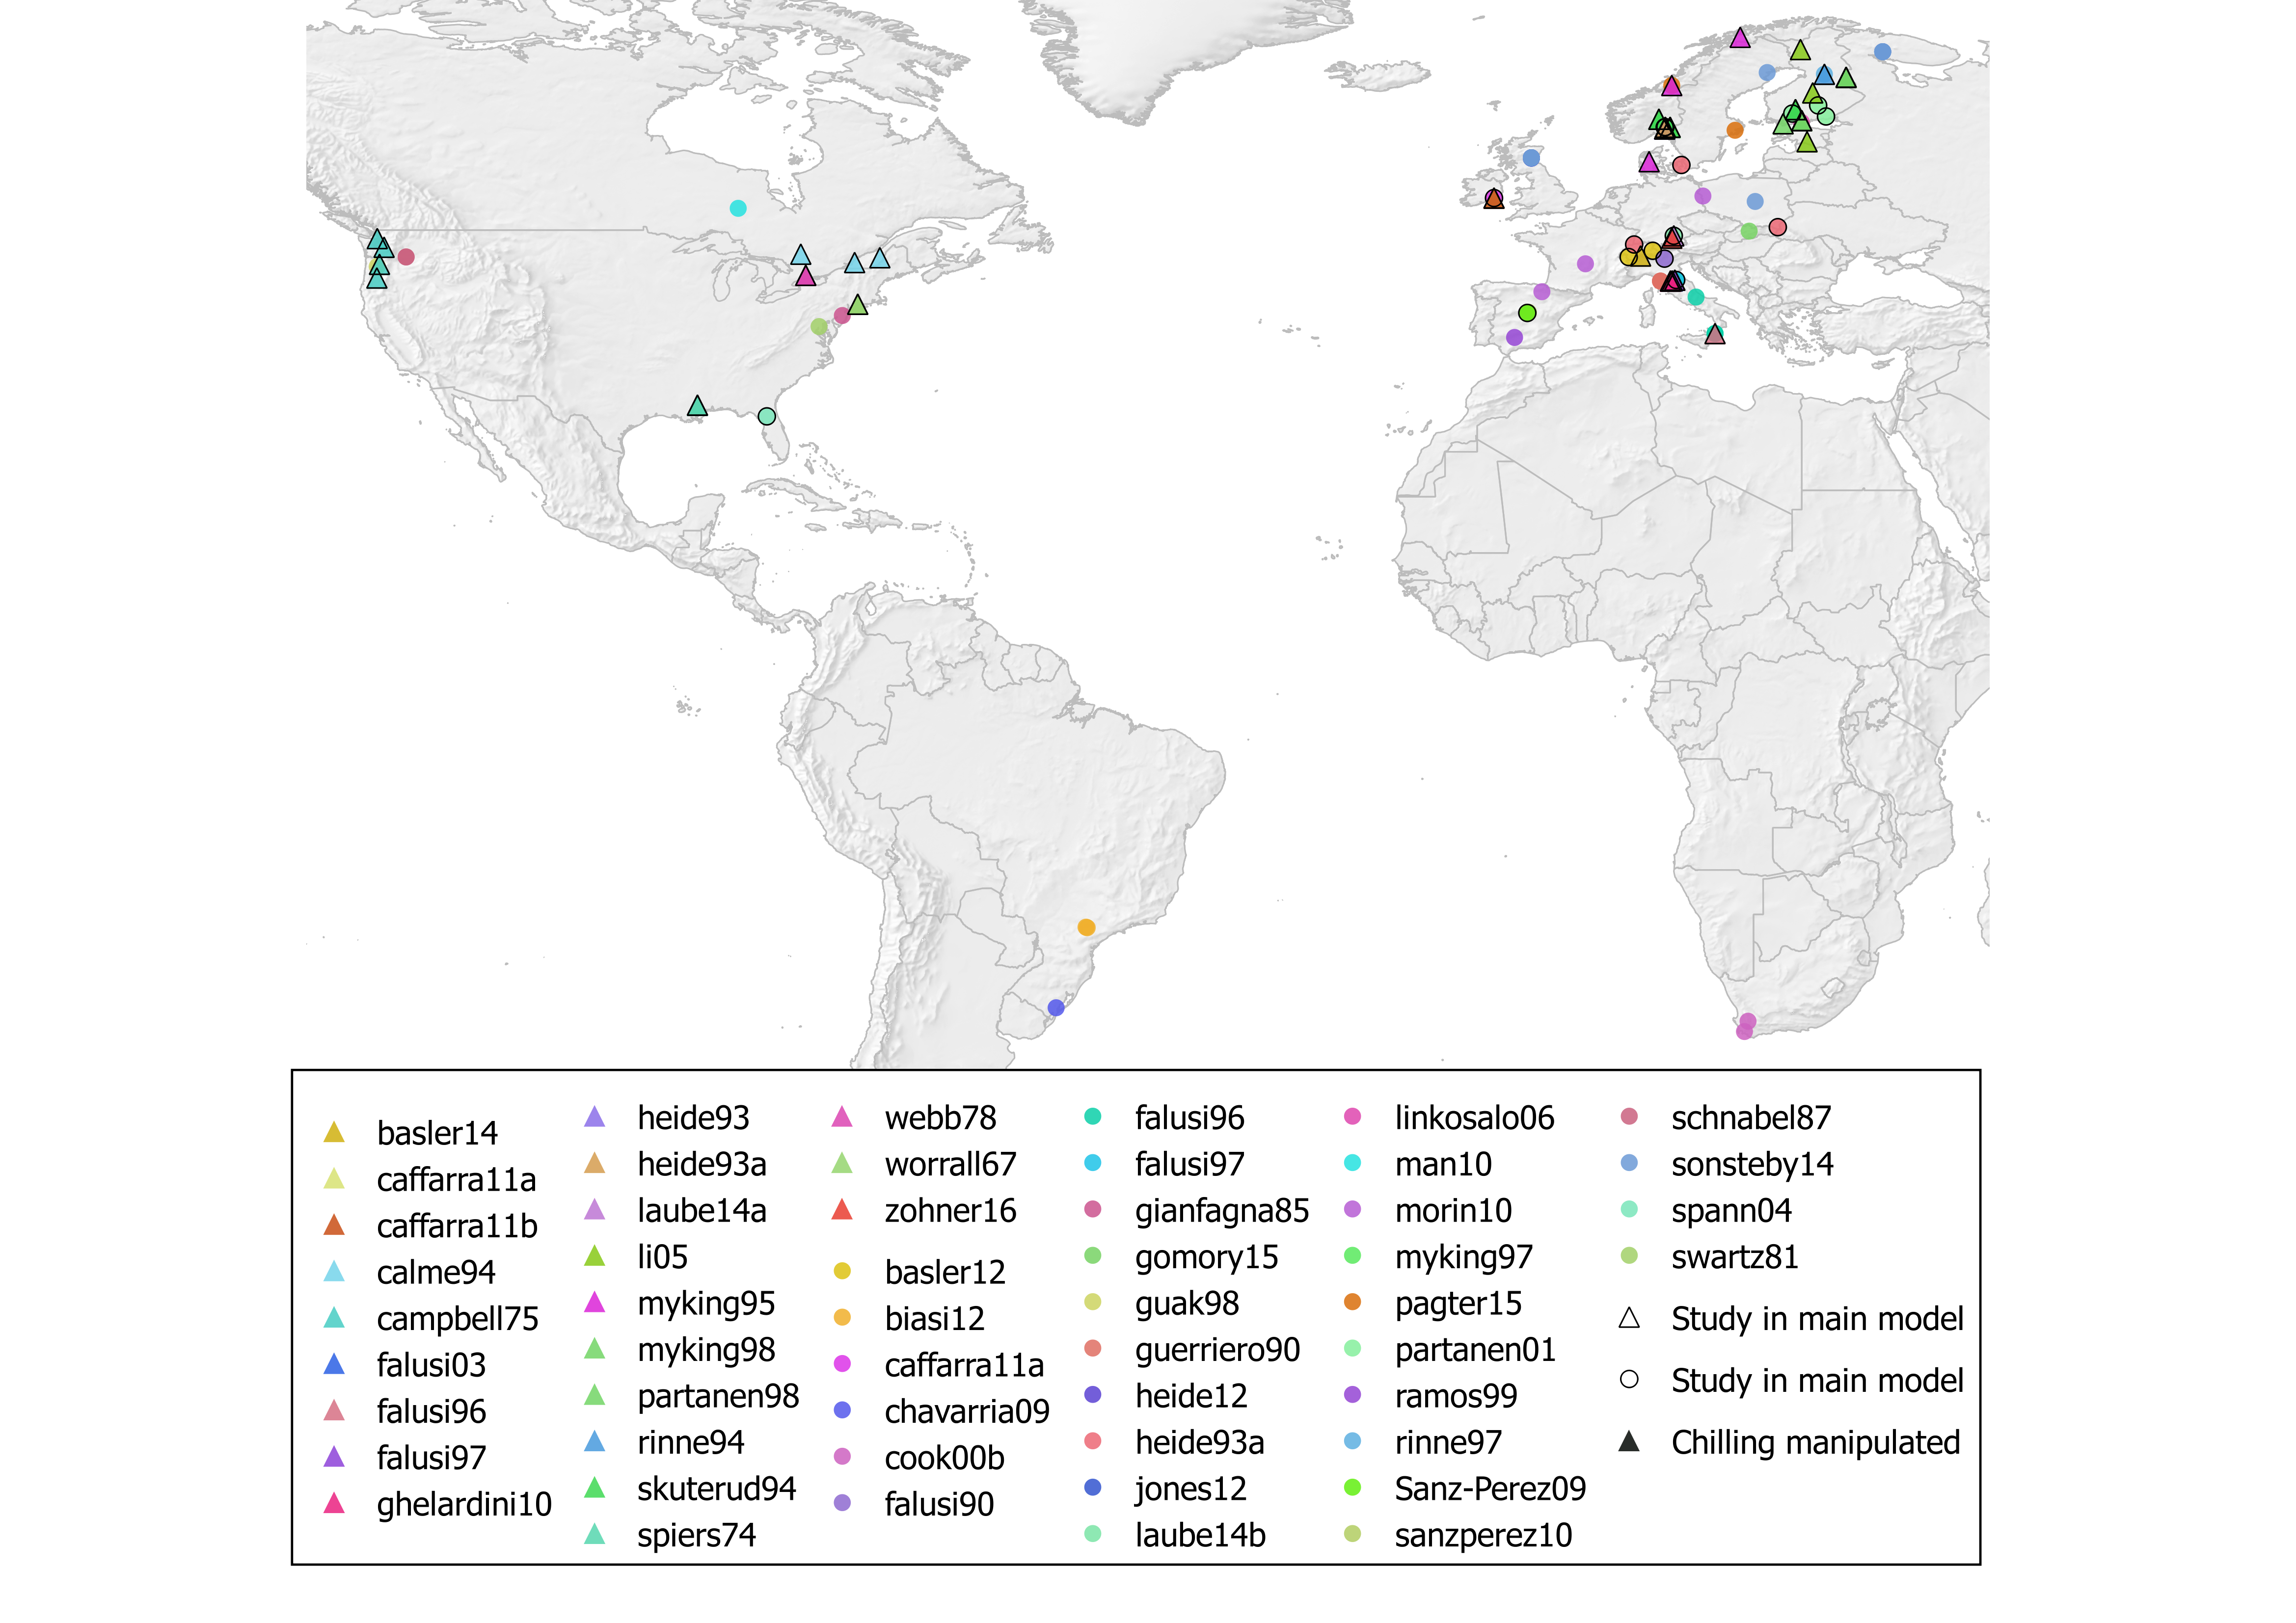
\includegraphics[width=0.9\textwidth]{..//..//analyses/bb_analysis/figures/ospree_locations_definitive.png}
\caption{\textbf{Map of days to budburst experiments in the OSPREE database.} Legend shows each dataset included in the main OSPREE model with all species and treatments (Tables \ref{tab:modsz}, \ref{tab:modsnonz}); symbols outlined in black represent datasets for which chilling was manipulated experimentally or through multiple field sample dates. See Table \ref{tab:ref} for the reference associated with each dataset.}
\label{fig:map}
\end{figure}


\begin{figure}[h!]
\centering
\noindent 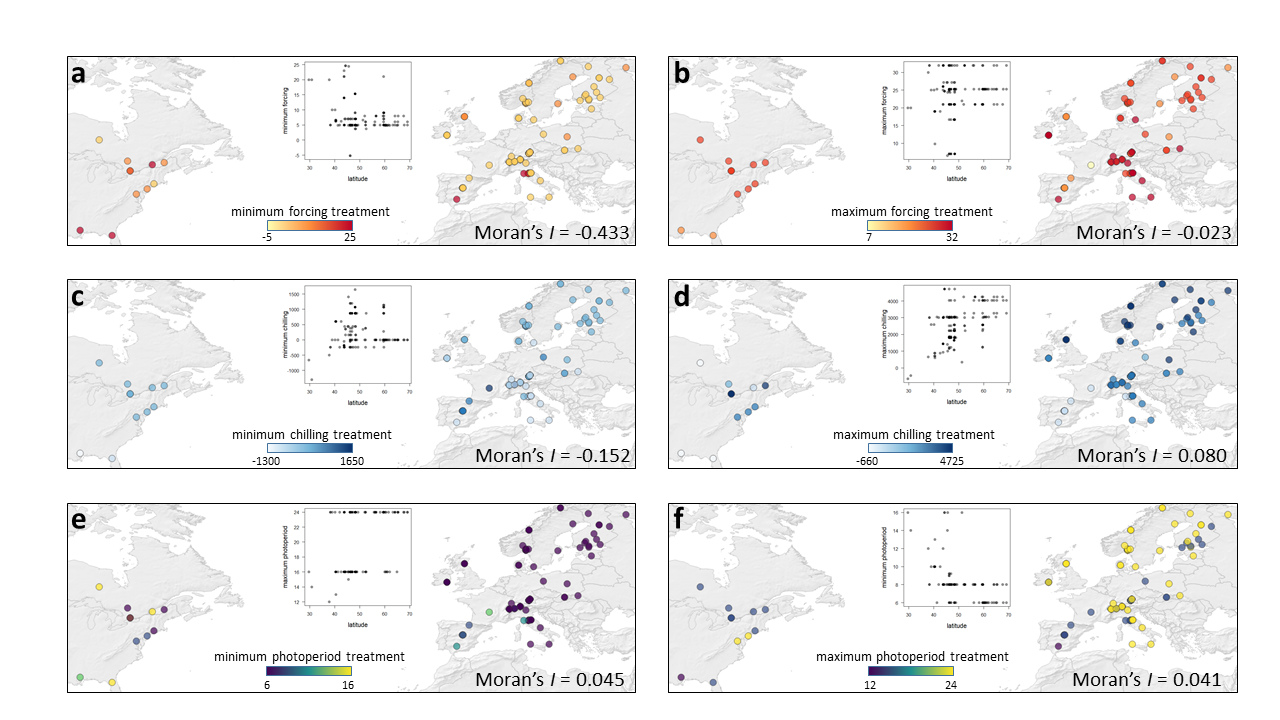
\includegraphics[width=0.9\textwidth]{..//..//analyses/bb_analysis/figures/minmaxtreatmentsmap.png}
\caption{\textbf{Map of chilling, forcing, and photoperiod treatments} across all species' days to budburst responses included in our main model, and the locations where each controlled environment experiment was conducted. We did not find strong spatial patterns in either minimum (a,c,e) or maximum (b,d,f) treatments, as measured by Moran's \emph{I}; insets show relationship of each cue's treatment level with the latitude of the experiment.}
\label{fig:trtmap}
\end{figure}

\newpage
\begin{figure}[h!]
\centering
\noindent 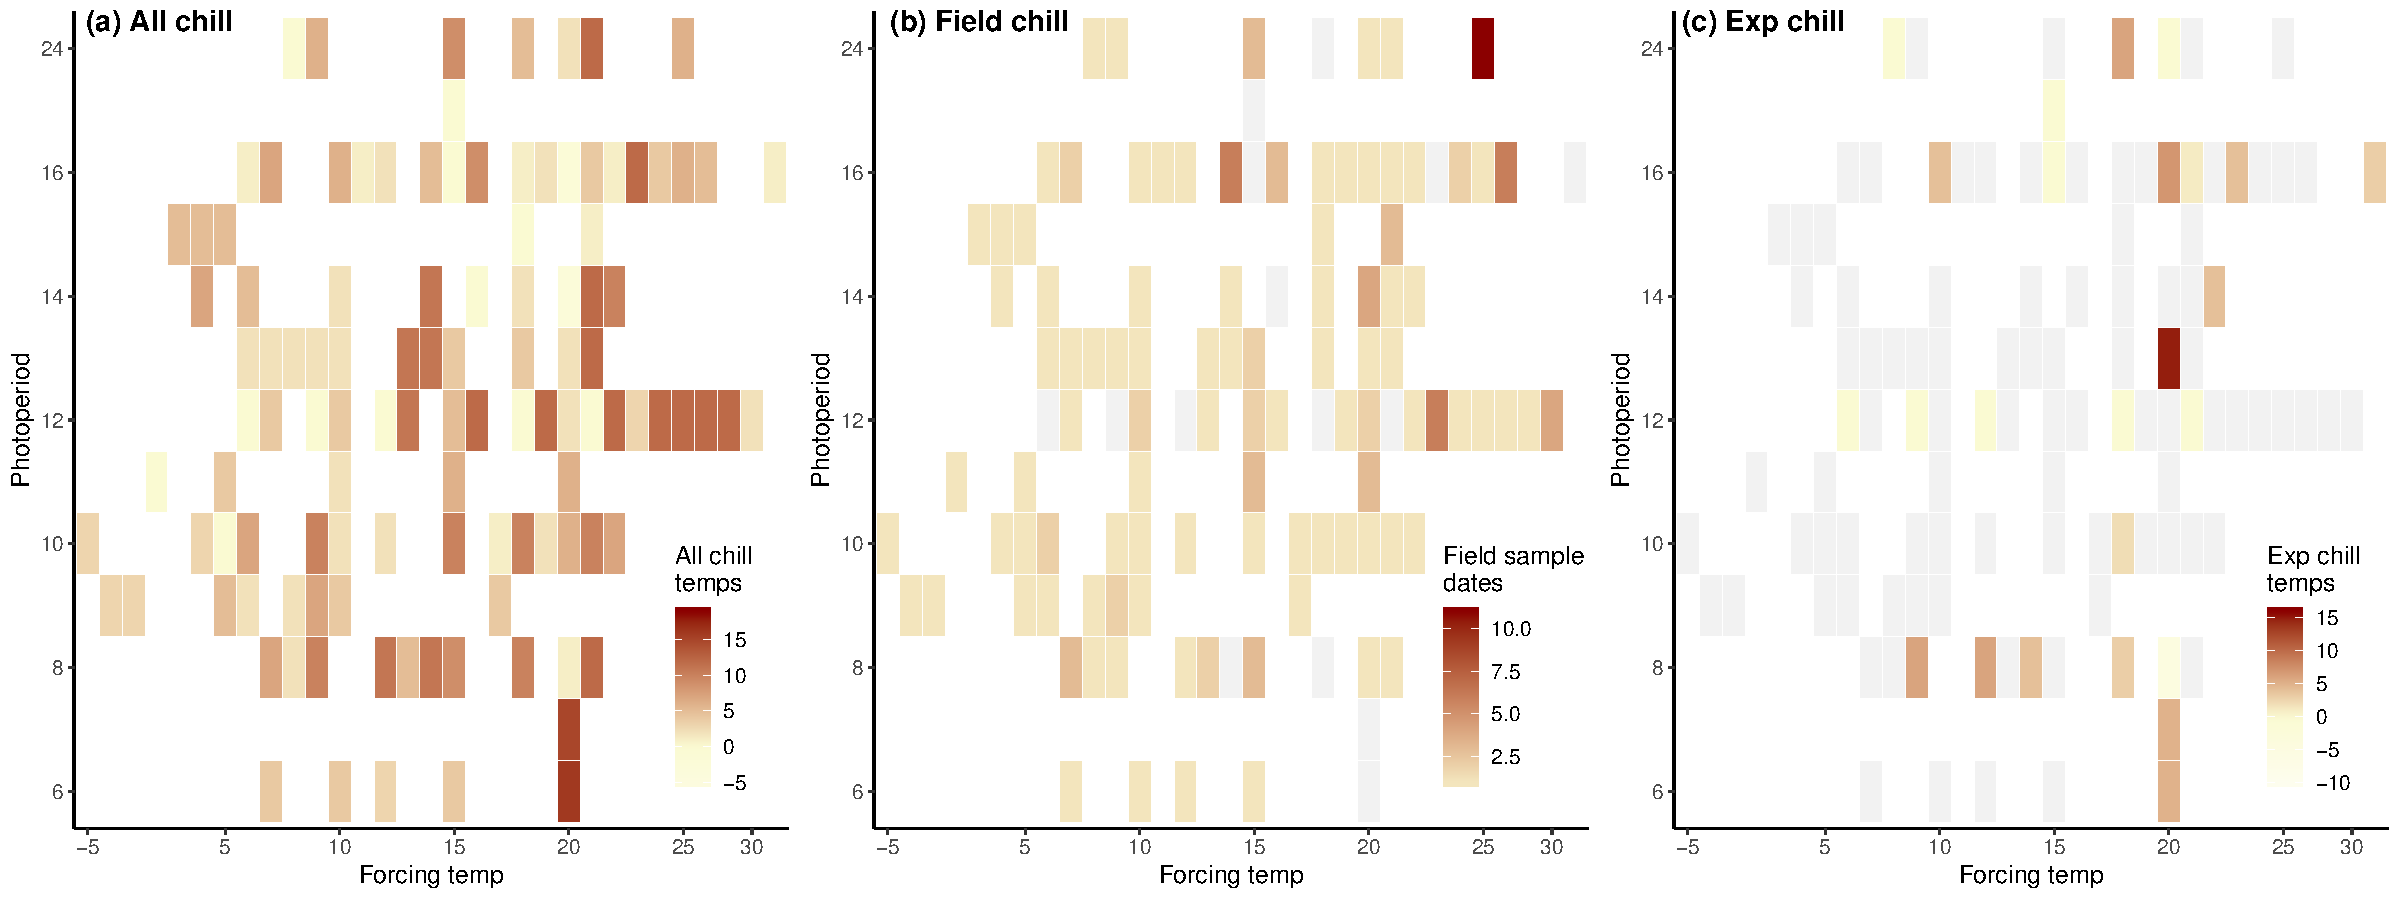
\includegraphics[width=0.9\textwidth]{..//..//analyses/bb_analysis/figures/studydesign/studydesign_heat3panelallsppmodel.pdf}
\noindent 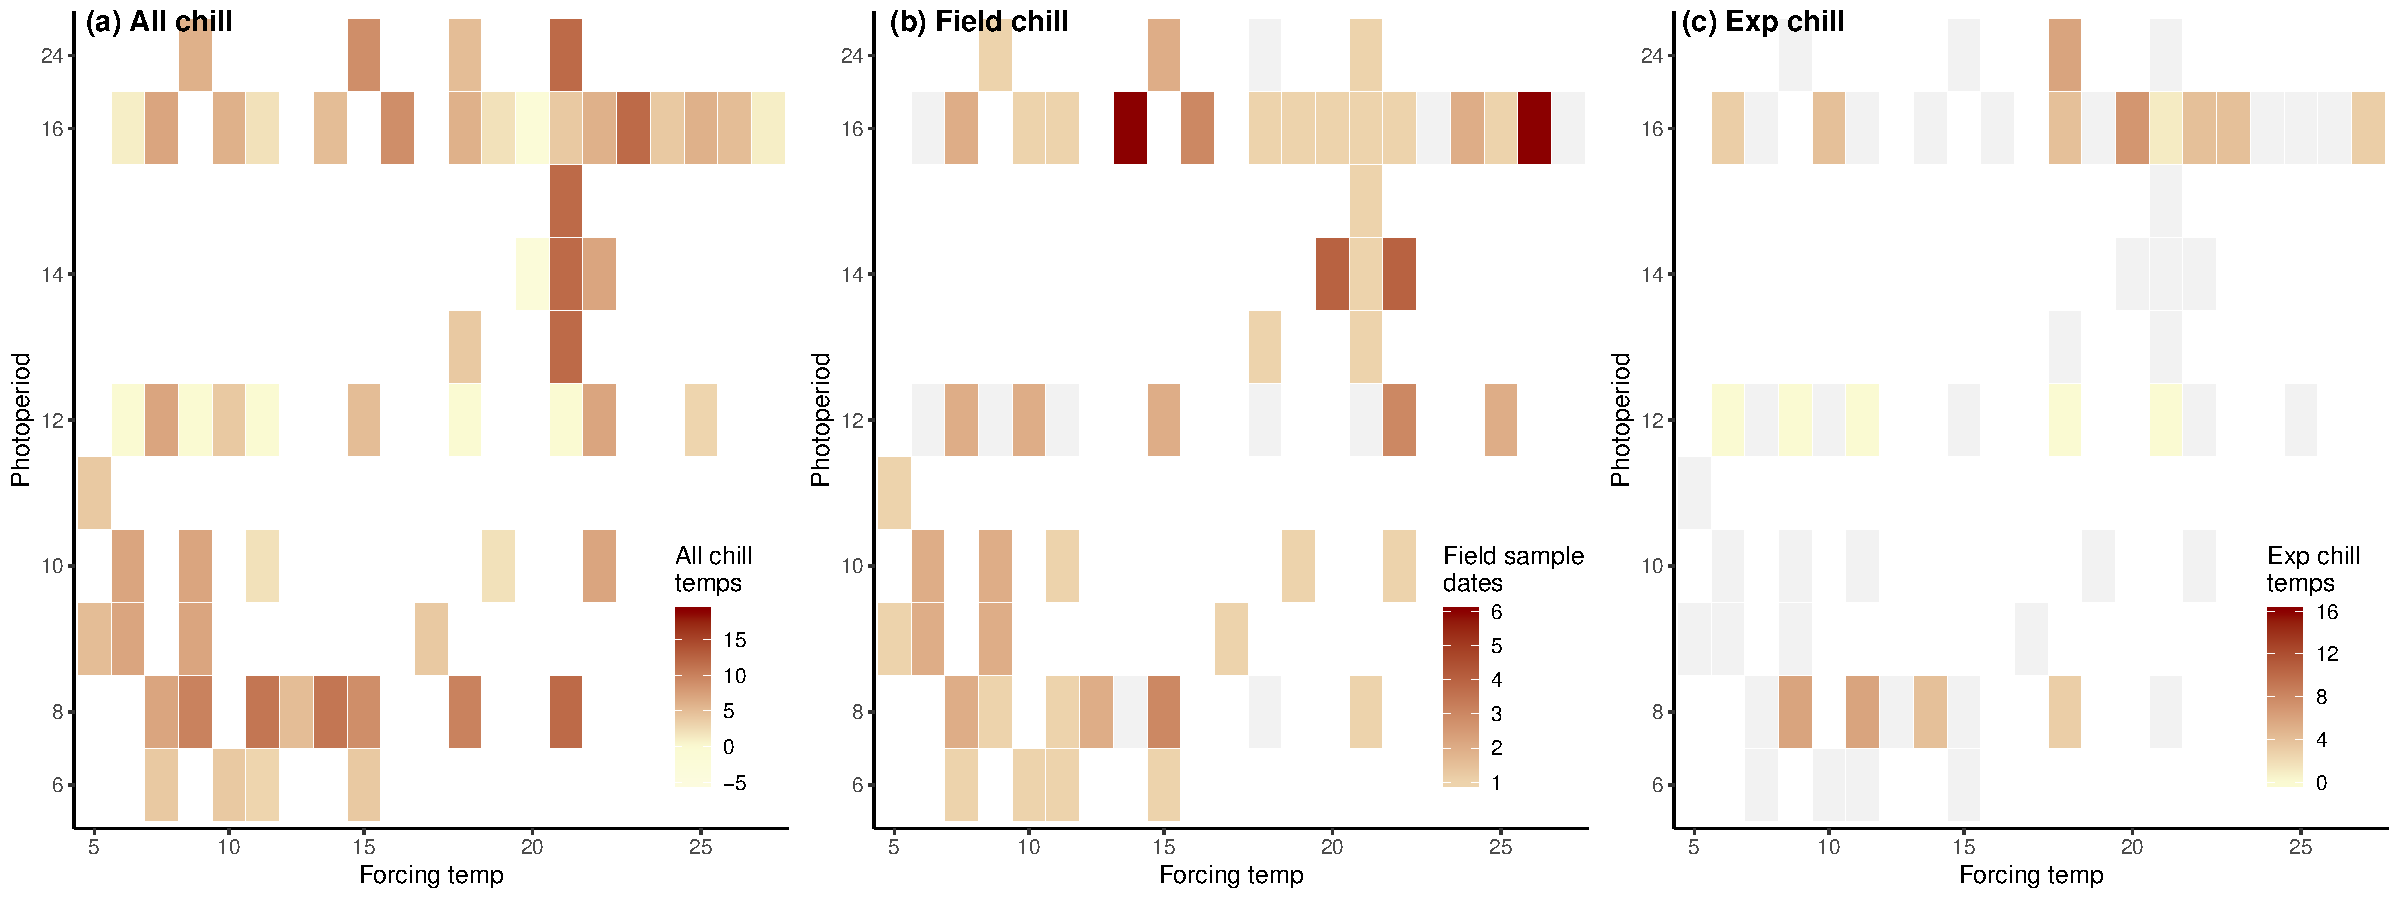
\includegraphics[width=0.9\textwidth]{..//..//analyses/bb_analysis/figures/studydesign/studydesign_heat3panelmainmodel.pdf}
\caption{\textbf{The diversity of study designs used in analyses.} Heatmaps show the range and commonness of different forcing (x-axis in all panels) by photoperiod (y-axis in all panels) combinations and with which chilling they were combined. In (A, top and bottom) we show our estimated chill units, which integrate across field (B, top and bottom) and experimental chilling (C, top and bottom). The top row shows all data included in the full model with 203 species, while the bottom row shows the data included in the main model with a subset of species well-represented across treatments and studies. Gray squares indicate a treatment was not applied (\emph{i.e.}, the prevalence of gray squares in (C) highlights how few studies include experimental chilling). Field sample dates are counted as any reported sampling dates more then 14 days apart.}
\label{fig:treatheatmaps} % see bb_analysis/studydesignplotsbb.R 
\end{figure}

\begin{figure}[h!]
\centering
\noindent 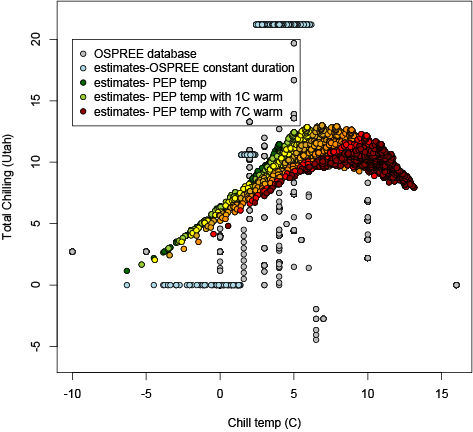
\includegraphics[width=0.50\textwidth]{..//..//analyses/bb_analysis/figures/exp_vs_field_chill_withwarmingcols.png}
\caption{\textbf{Chilling accumulates differently in experiments with constant temperatures versus natural systems}, in which temperature is more strongly correlated with chilling. See \emph{Estimating chilling} for a detailed description of ``Field'' climate data, for which we use historical climate data from Europe. Fig. \ref{fig:3dfieldchillutah} uses ``Field'' relationships to convert chill temperature to total chilling, whereas Fig. \ref{fig:3dexpchillutah} uses 'Constant duration' relationships.}
\label{fig:chillexpfield}
\end{figure}

 \begin{figure}[h!]
 \centering
 \noindent 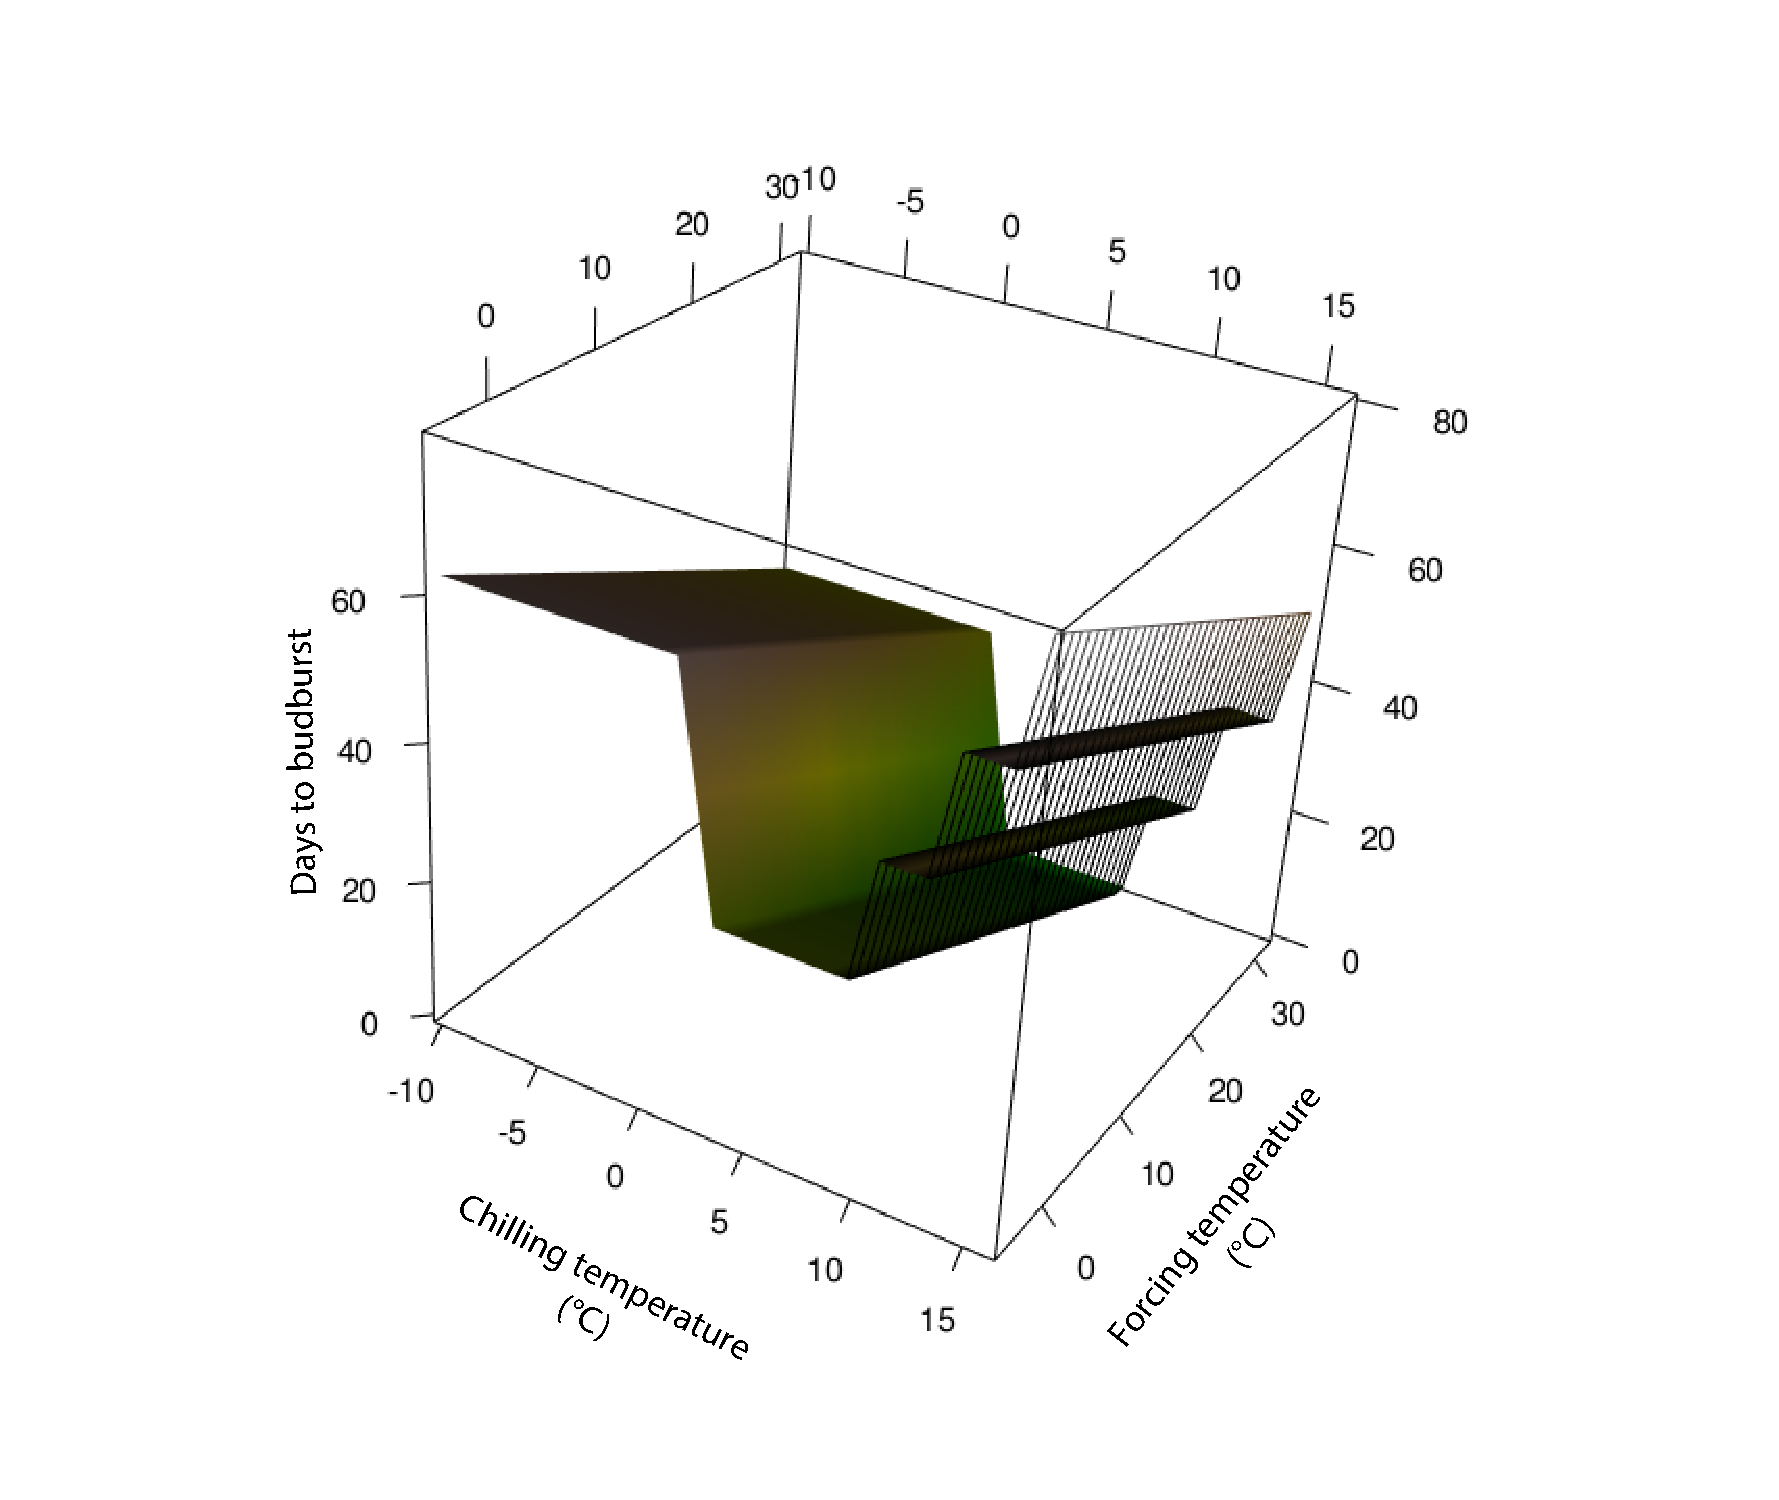
\includegraphics[width=0.75\textwidth]{..//..//analyses/bb_analysis/figures/bbmod_3dplot_utah.pdf}
 \caption{\textbf{Estimates of budburst across a range of forcing temperatures and estimated chilling} (converted to a representative mean temperature, see \emph{Estimating chilling} in the Supplemental Materials) based on overall estimates of chilling and forcing effects (Fig. \ref{fig:mu}). Maximum advances in budburst occur at intermediate chilling temperatures (\emph{e.g.}, here at mean winter temperatures of 6-7\degree C) and the highest forcing (here at 32\degree C). We set photoperiod to eight hours, which is the most common photoperiod treatment in the database. Note that days to budburst is relative to experimental methods and thus is not comparable to day of year in the field; shading represents days to budburst. Compare this to Fig. \ref{fig:3dfieldchillutah} in the main text.} 
 \label{fig:3dexpchillutah}
 \end{figure}
 \newpage


\begin{figure}[h!]
\centering
\noindent 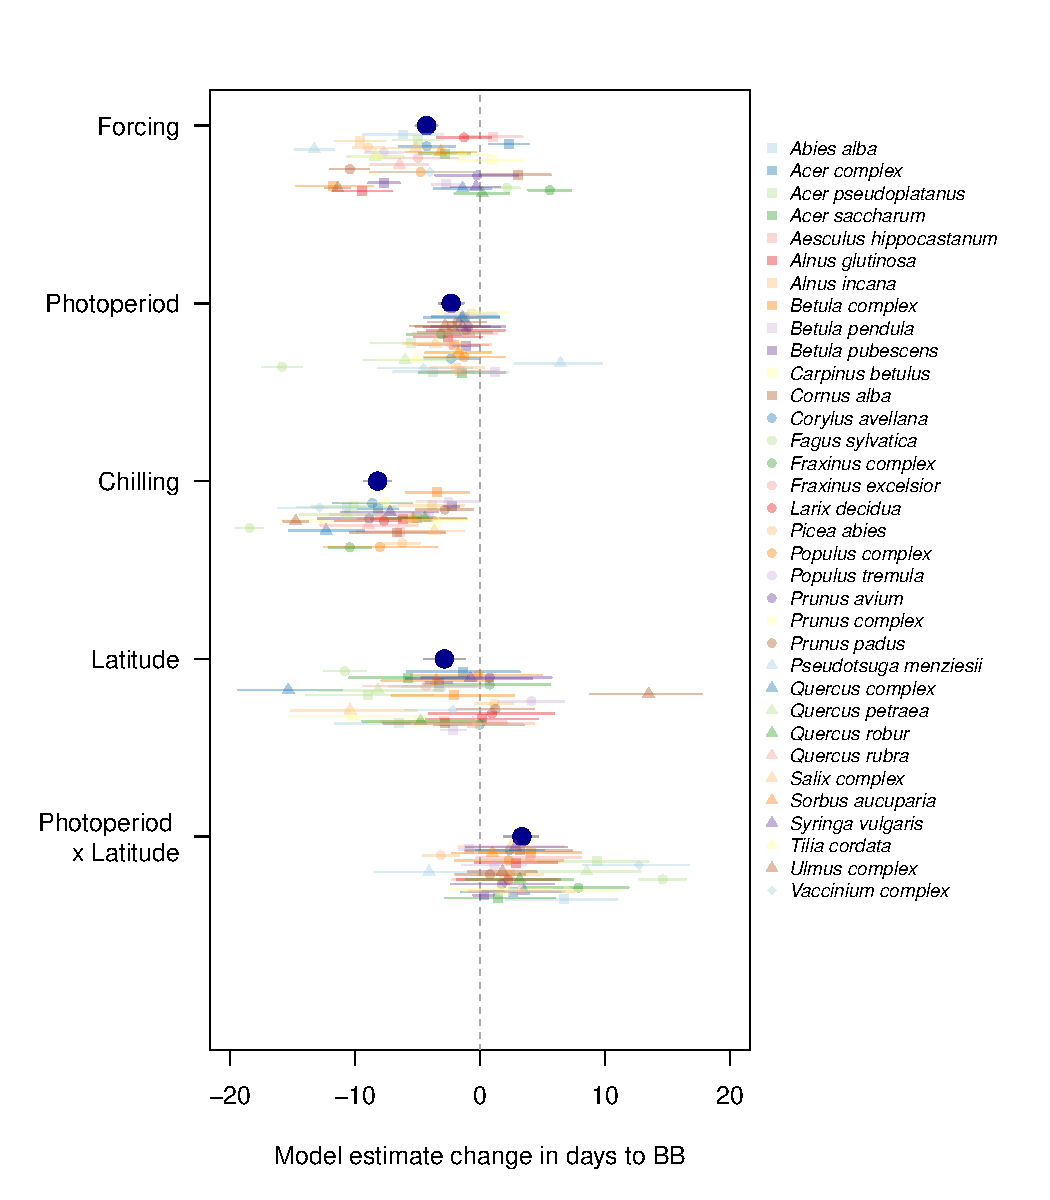
\includegraphics[width=0.75\textwidth]{..//..//analyses/lat_analysis/figures/latanalysis_spcom_expramp_fp.pdf}
\caption{\textbf{Estimates for effects of chilling exceeded estimates for forcing, photoperiod, provenance latitude, and the interaction between latitude and photoperiod, for most species,} in the latitude budburst model, using Utah units (Table \ref{tab:lat}). Using standardized units, which allow comparisons across cues, we show that, as with the main budburst model (Fig. \ref{fig:concept}), most species (smaller symbols) are responsive to most cues. Chilling is the strongest cue when considering overall estimates across species (larger, dark blue circles).}
\label{fig:lat}
\end{figure}


\begin{figure}[h!]
\centering
\noindent 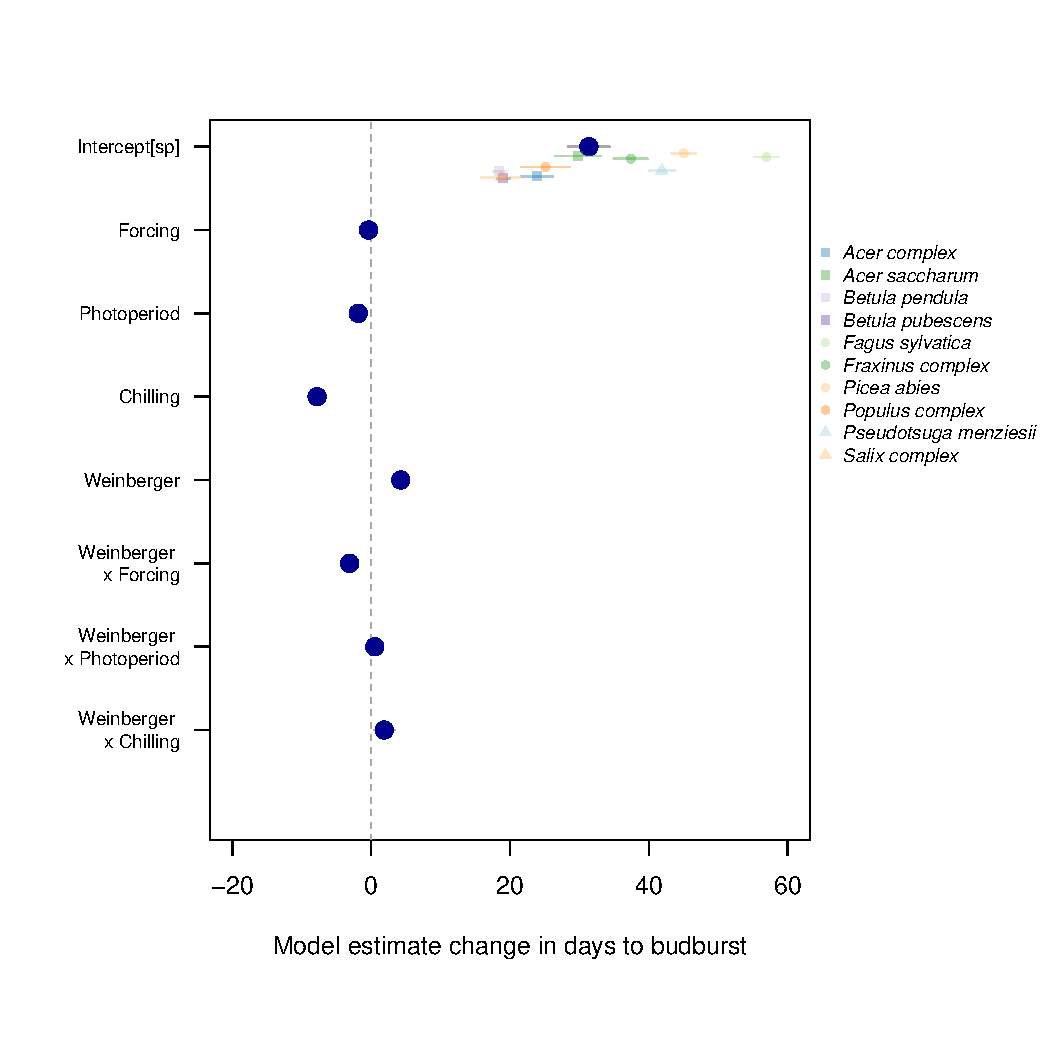
\includegraphics[width=0.75\textwidth]{..//..//analyses/figures/weinberger_MU_4supp.pdf}
\caption{\textbf{Chilling study design affects estimates of major cues.} Studies using the ``Weinberger'' method (sequential removal of tissue from field) had later budburst timing, stronger estimates of forcing (Weinberger x Forcing) and weaker estimates of chilling (Weinberger x Chilling) compared to studies that experimentally manipulated chilling directly. For an extended description of model and underlying data see \emph{Chilling study design model}; for model summary see Table \ref{tab:methods}.}
\label{fig:weinberger}
\end{figure}

\begin{figure}[h!]
\centering
\noindent 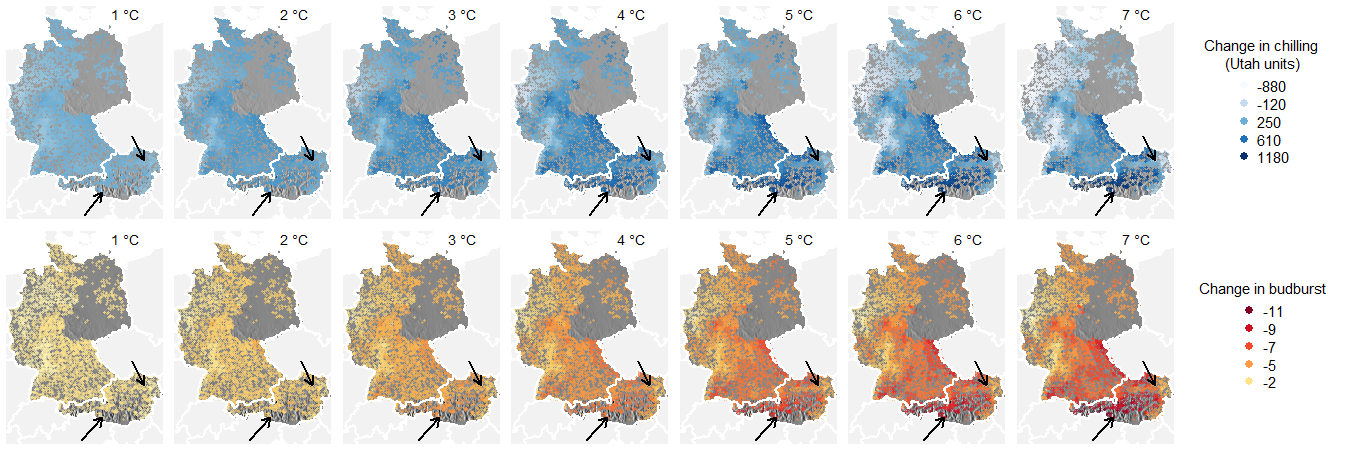
\includegraphics[width=0.90\textwidth]{..//..//analyses/bb_analysis/figures/forecasting/heatmapsbetpepfinalarrows.png}
\caption{\textbf{Forecasted changes in chilling (top panel) and spring phenology for \emph{Betula pendula} (bottom panel)}, in locations included in the PEP725 database, where phenology dates are known for the pre-warming time period (1951-1960). Changes in chilling and budburst are calculated relative to the mean chilling and leafout dates during this pre-warming time period for each location. Arrows indicate sites shown in Fig. 3A (latitude = 46.8\degree N, longitude =  12.8\degree E, 659 m above sea level) and 3B (latitude = 48.3\degree N, longitude =  15.8\degree E, 210 m above sea level) in the main text.} 
\label{fig:foremap}
\end{figure}

\begin{figure}[h!]
\centering
\noindent 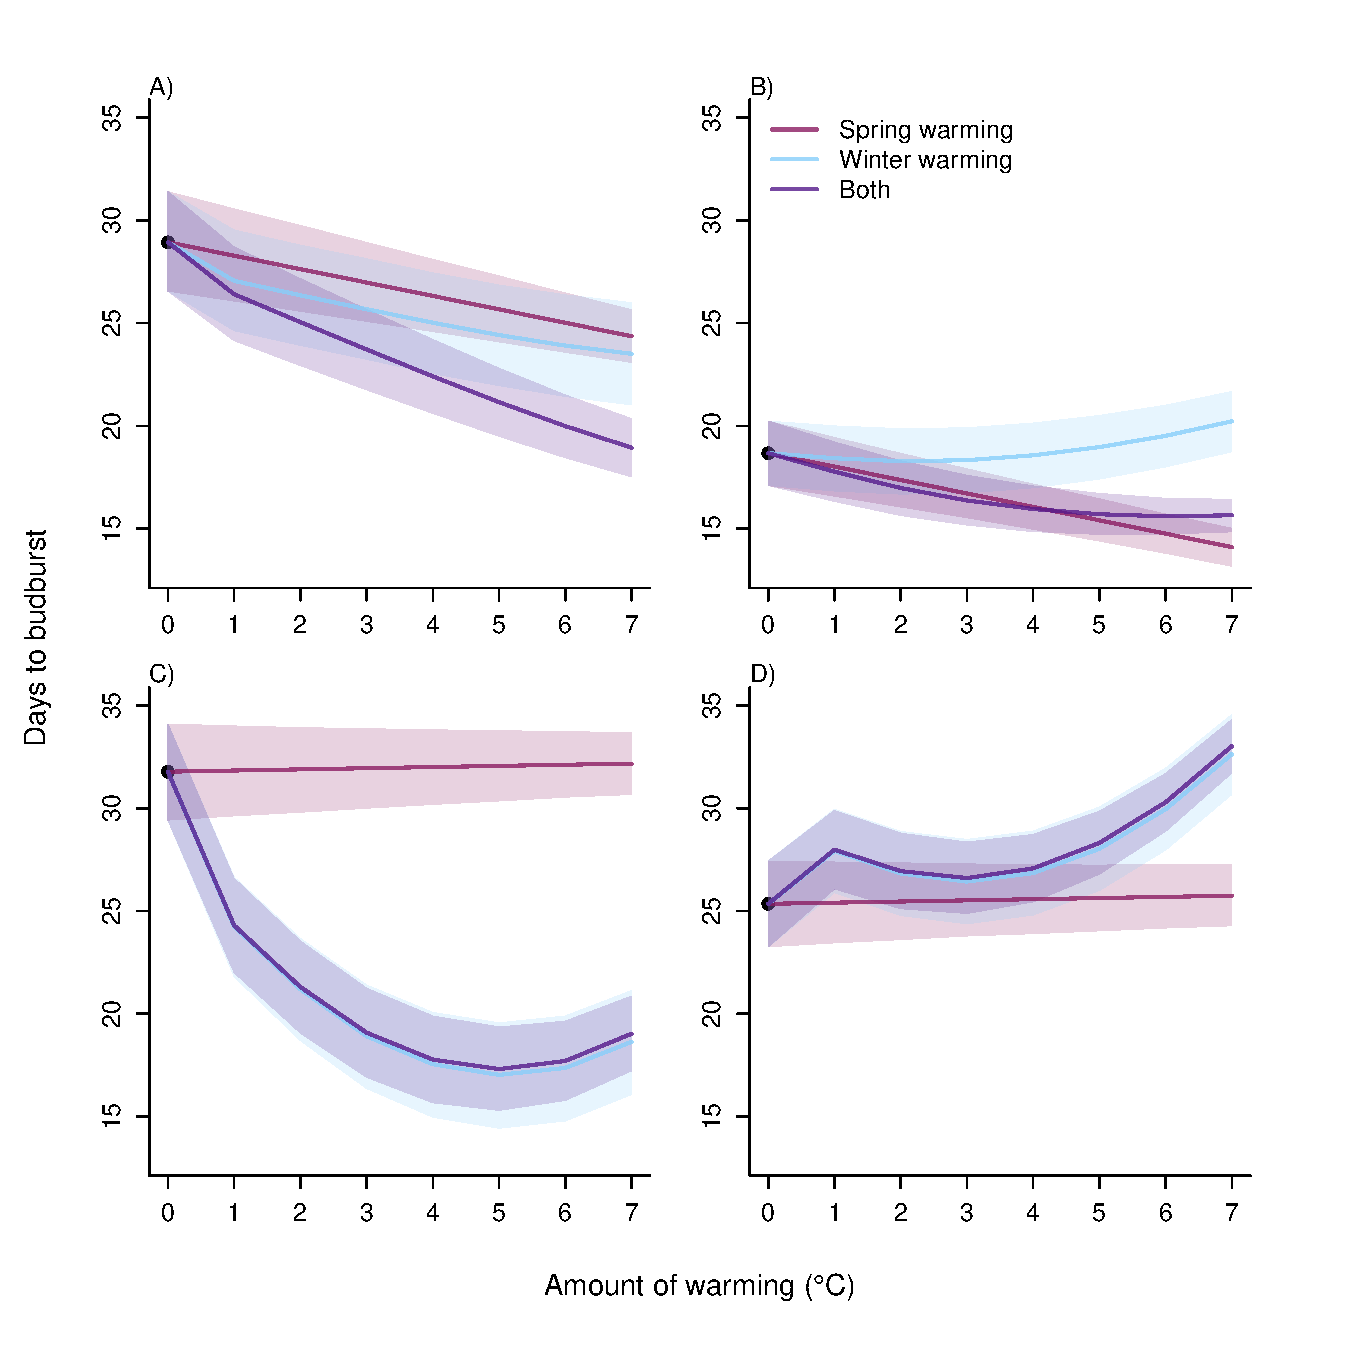
\includegraphics[width=0.75\textwidth]{..//..//analyses/bb_analysis/figures/forecasting/tempforecastbothspp_1_7_degwarm.pdf}
\caption{\textbf{Implications of warming on budburst timing varies across species and sites}, depending strongly on pre-warming climate conditions related to chilling for each site. Here we show species-level estimates from our model (Fig. \ref{fig:mu}) for the two most common species in the OSPREE database: \emph{Betula pendula} (A, B) and \emph{Fagus sylvatica} (C, D), for sites that highlight the diversity of possible budburst responses to warming (Fig. \ref{fig:foremap}, which shows general trends across many sites in Central Europe). In some sites, warming increases total chilling estimates (A, C) leading to greater advances in budburst (compared to forcing alone), whereas warming decreases total chilling estimates in other sites (B, D), leading to smaller advances and, eventually, delays with substantial warming. Compare this Fig. \ref{fig:3dfieldchillutah} in the main text, which shows all possible combinations of winter and spring warming in a three-dimensional plot.}
\label{fig:betfag2d}
\end{figure}

\begin{figure}[h!]
\centering
\noindent 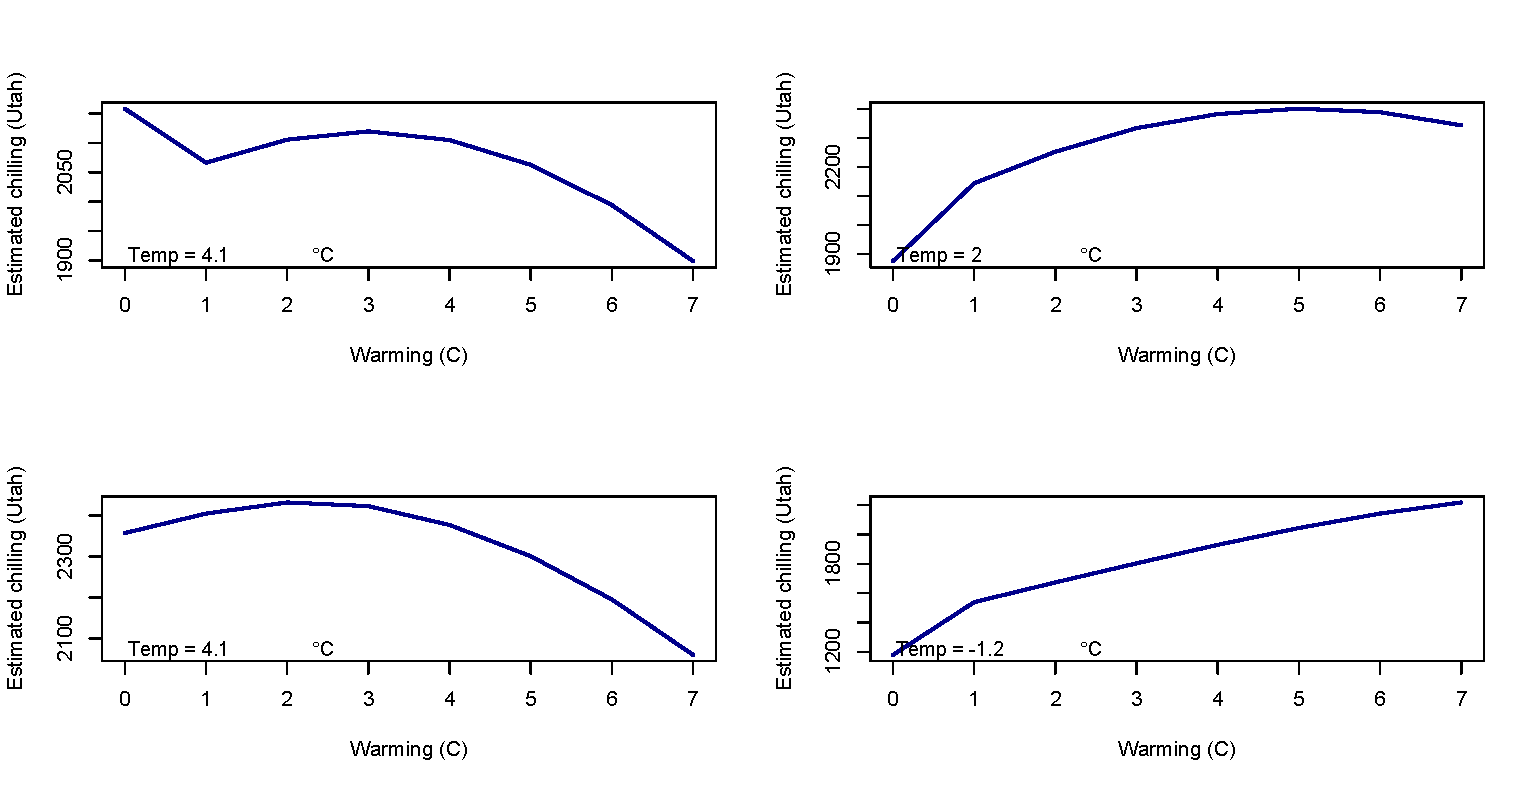
\includegraphics[width=0.75\textwidth]{..//..//analyses/bb_analysis/figures/forecasting/chillforecast_bothspp_PEP_utah.pdf}
\caption{\textbf{Implications of global warming on chilling vary by site}, depending on pre-warming climate. For sites in A (lat, lon) and D (lat, lon), chilling increases with warming, whereas chilling decreases with warming for the sites in B (lat,lon) and C (lat,lon). Compare to Fig. \ref{fig:betfag2d} and Fig. \ref{fig:3dfieldchillutah} in the main text.}
\label{fig:chillfore}
\end{figure}

\begin{figure}[h!]
\centering
\noindent 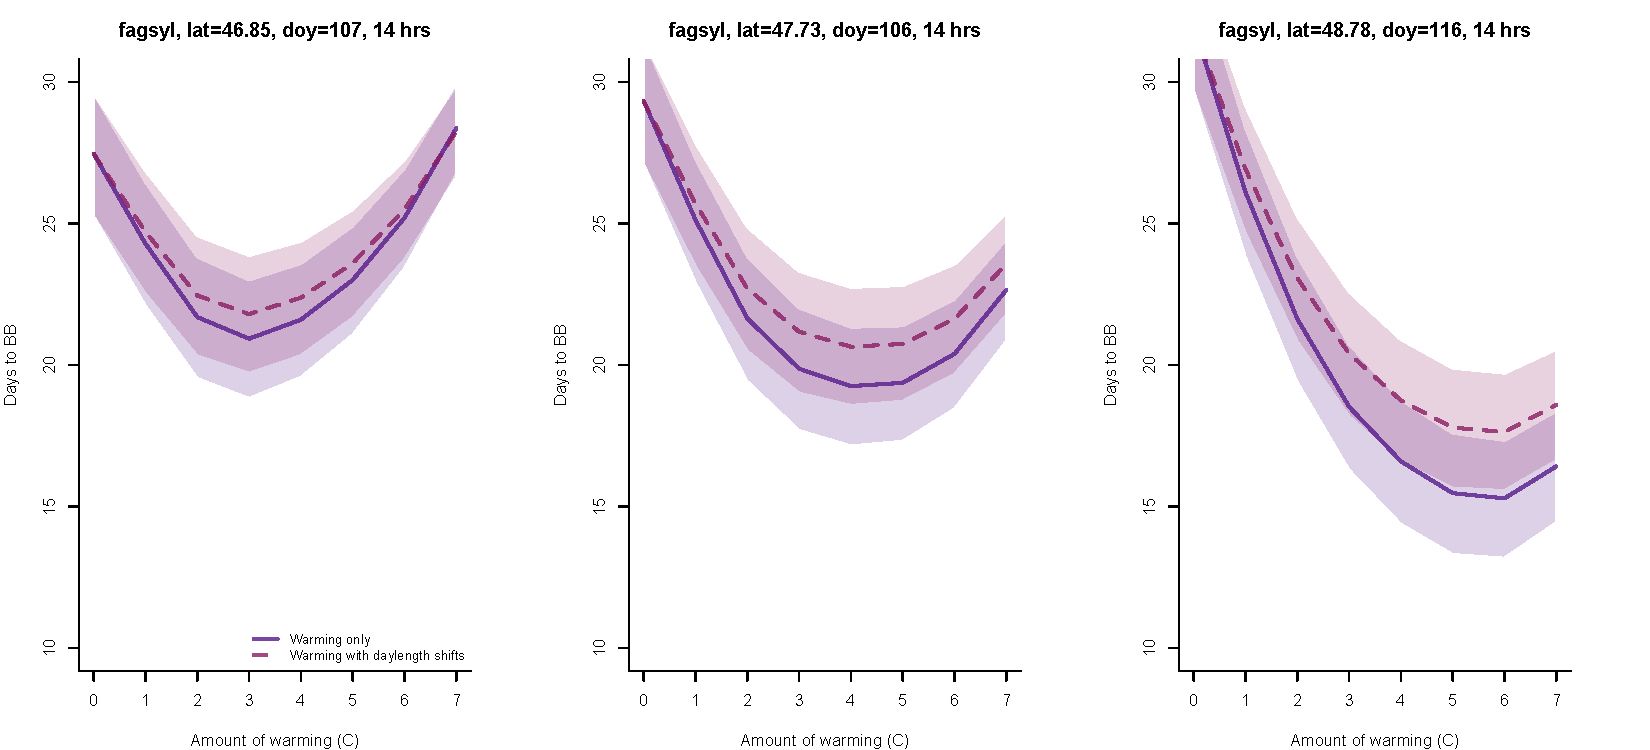
\includegraphics[width=0.75\textwidth]{..//..//analyses/bb_analysis/figures/forecasting/fagsyl_3lats.pdf}
\caption{\textbf{Budburst is affected by climate-change induced shifts in photoperiod, especially at high latitudes}, though effects vary by site and are minor compared to effects of warming. We show forecasted effects of varying levels of warming on \emph{Fagus sylvatica}, the most photoperiod-sensitive species in our database, across three latitudes within its range, as predicted by the latitude model. The low latitude site (A) is  located at 46.8\degree N, 15.7\degree E; the mid-latitude site (B) is located at 47.7\degree N, 16.3\degree E; and the high-latitude (C) site is located at 48.8\degree N, 15.4\degree E.}
\label{fig:fagsyllat}
\end{figure}

\newpage
\begin{figure}[h!]
\centering
\noindent 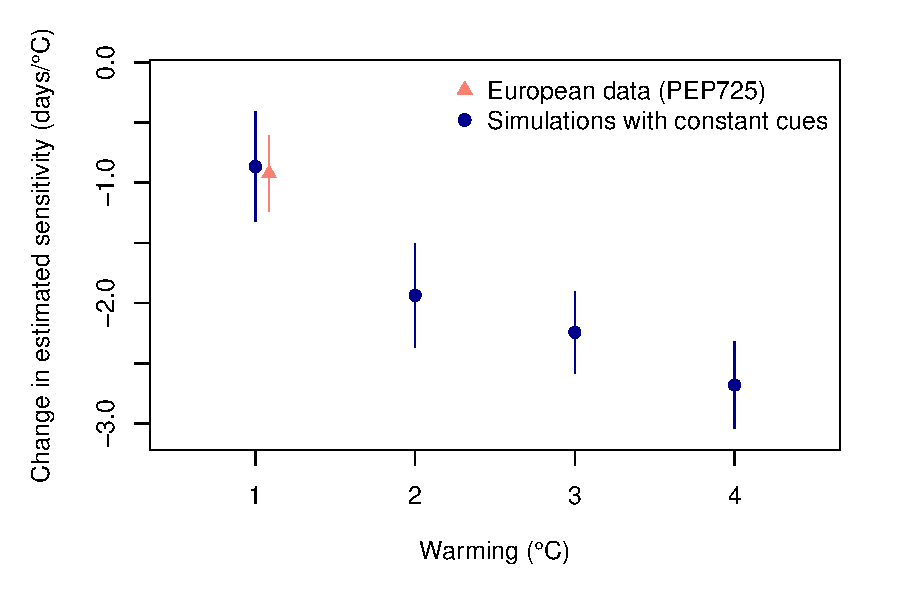
\includegraphics[width=0.75\textwidth]{..//..//analyses/bb_analysis/PEP_climate/figures/peprealandsims.pdf}
\caption{\textbf{Declining sensitivities observed in long-term European data for a suite of common trees may be explained by a statistical artifact.} We compared the sensitivity estimated from linear regressions of day of leafout versus mean spring temperature (estimated thus as days/$^{\circ}$C) from PEP725 data for \emph{Betula pendula} from 45 sites (``European data'') with estimated declines in simulations where the cues were held constant but spring temperatures warmed by 1-4$^{\circ}$C (``Simulations'') and found the estimated temperature sensitivity measured as days/$^{\circ}$C declined even though the underlying cues had not changed, see \emph{Understanding declines in temperature sensitivity in European long-term data} for further details.}
\label{fig:pepsims}
\end{figure}

\newpage
\begin{figure}[h!]
\centering
\noindent 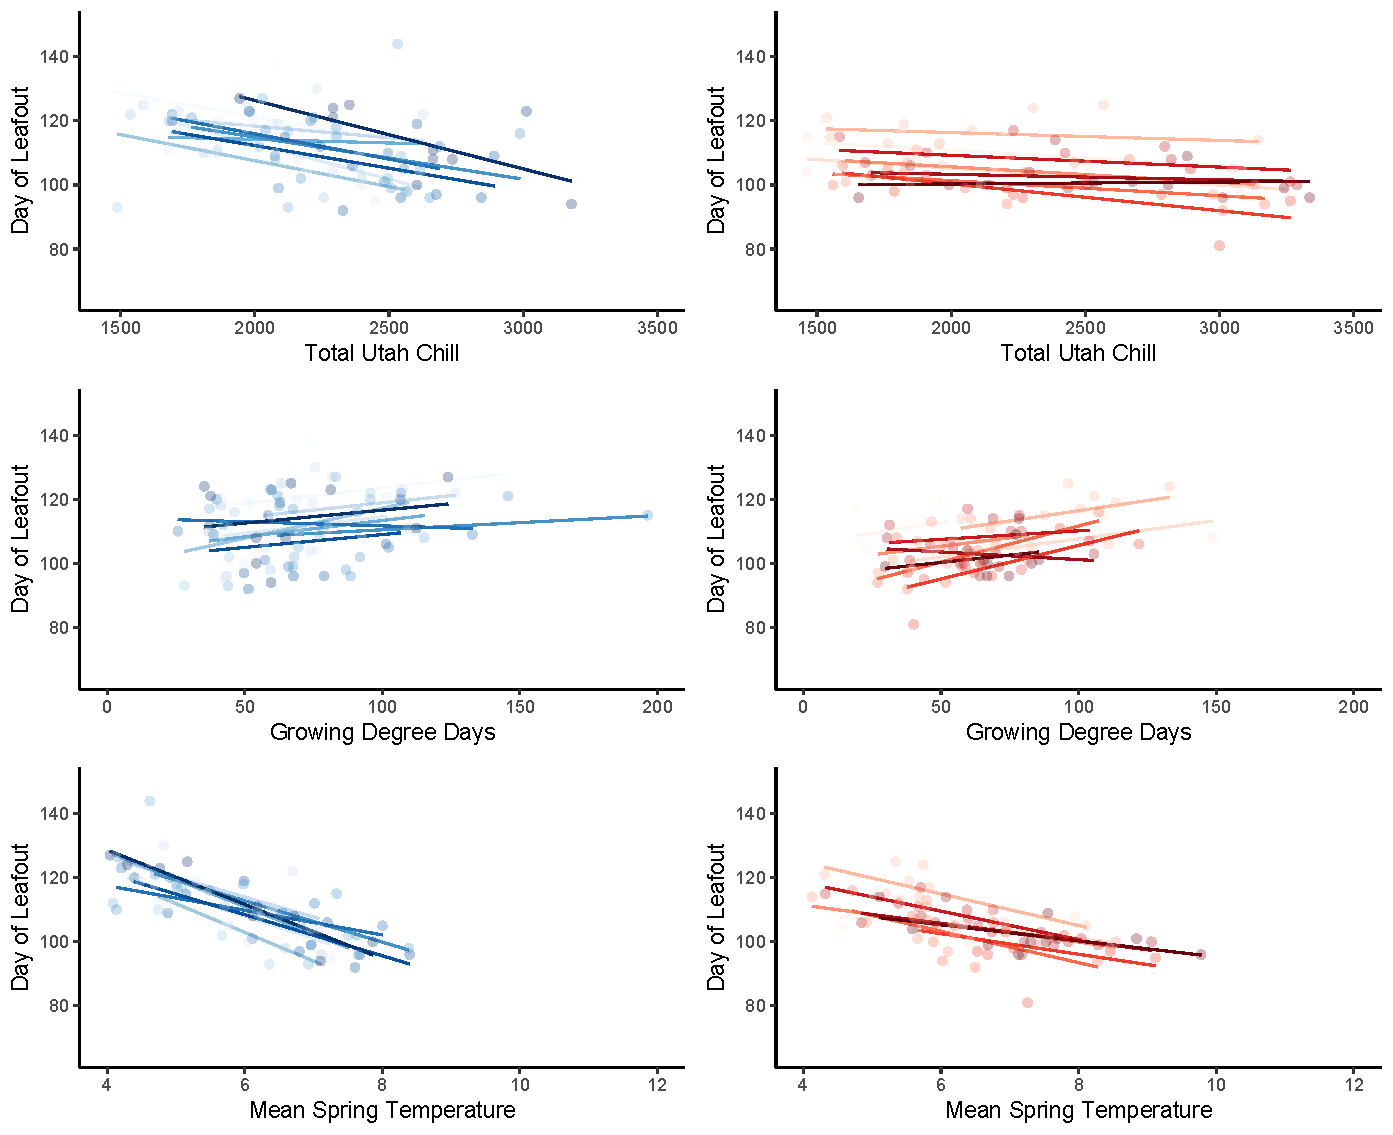
\includegraphics[width=0.75\textwidth]{..//..//analyses/bb_analysis/PEP_climate/figures/betpen_multruns_utahgddmat.pdf}
\caption{\textbf{Day of leafout versus chilling, growing degree-days, and mean spring temperature} pre- (left panels, 1951-1960) and post-warming (right panels, 2000-2010) for PEP725 sites in Germany where \emph{Betula pendula} phenology has been monitored for decades.}
\label{fig:pep}
\end{figure}

\begin{figure}[h!]
\centering
\noindent 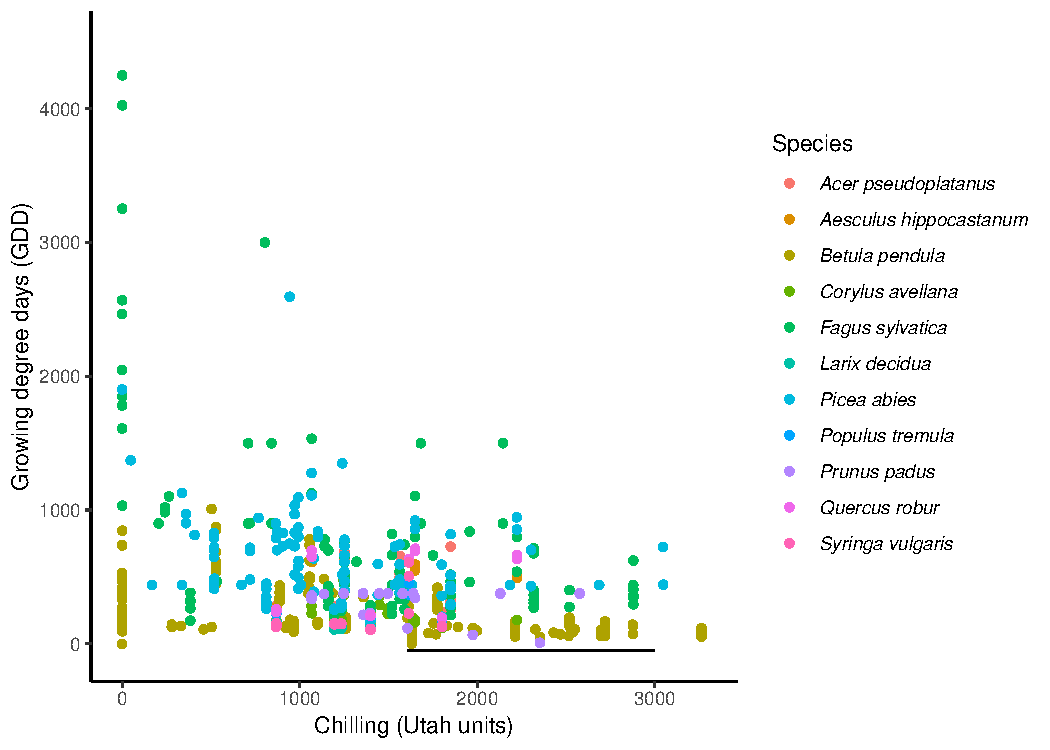
\includegraphics[width=1\textwidth]{..//..//analyses/bb_analysis/figures/gddbyutah_pepspp.pdf}
\caption{\textbf{Growing degree days (GDD) versus chill units at the time of budburst} from the OSPREE database for common species in the PEP725 long-term phenological database. The black line shows the range of chilling (10-90\% quantiles) accumulated from 1 September to 1 March for 45 sites for \emph{Betula pendula} (see also \emph{Understanding declines in temperature sensitivity in European long-term data}). We calculated GDD here as the average daily forcing temperature multiplied by days to budburst.}
\label{fig:pepgddchill}
\end{figure}

%%%%%%%%%%%%%%%%%%%%%%%%%%%%%%%%%%%%%%%%
\end{document}
%%%%%%%%%%%%%%%%%%%%%%%%%%%%%%%%%%%%%%%%
